\chapter{Ejercicio de vuelta rápida de un Fórmula-1}\label{cap.chrono}
En este capítulo abordaremos todo lo relacionado con el desarrollo de una de las prácticas llamada \textit{Chrono}. Esta práctica formará parte del conjunto de ejercicios de \textit{Robotics-Academy}. Se explica la infraestructura de soporte de la práctica, las dos plantillas \textit{software}(una como nodo ROS y otra como cuadernillo Jupyter) y el funcionamiento de la solución de referencia desarrollada.

\section{Enunciado}\label{sec.enunciado}
Para el objetivo de esta práctica, el estudiante debe desarrollar un algoritmo que dote de la inteligencia necesaria a un modelo de robot F1 para que complete una vuelta con conducción autónoma en el menor tiempo posible. En el circuito hay pintada una línea roja para ayudar. El código del alumno compite con el récord grabado para el circuito. De esta manera, no solo se permite el desarrollo de un algoritmo funcional, sino que se propone un avance en el grado de dificultad exigiendo al alumno que optimice su algoritmo para que consiga completar una vuelta al circuito sin colisionar y con un tiempo inferior al ofrecido.

Para desarrollar la solución del algoritmo, el alumno deberá abordar distintos problemas. El primero de ellos es programar un filtrado de la imagen que capta el robot F1 por su cámara y escoger la línea roja central del circuito. Tras esto, el alumno deberá desarrollar un avance controlado del robot F1 para que siga la línea roja que ha sido filtrada.

Como puede observarse en los problemas abordados, además de tener que afrontarlos, es necesario que sean abordados conjuntamente, ya que el movimiento controlado del modelo depende del filtrado de las imágenes. Para añadir dificultad a la práctica, es necesario que el algoritmo de control de movimiento del vehículo sea eficaz dado que, de otro modo, será más lento que la solución proporcionada como referencia y llegará en segundo lugar.

\section{Infraestructura}
Este ejercicio funciona en un determinado escenario de \textit{Gazebo}, que ha habido que desarrollar y con un Fórmula-1 importado que ha tenido que ser modificado. El coche tiene una cámara, como sensor principal, y dos actuadores que permiten controlar su velocidad de giro y velocidad de tracción (Figura \ref{fig.infraestructura_ch}).

\begin{figure}[H]
  \begin{center}
    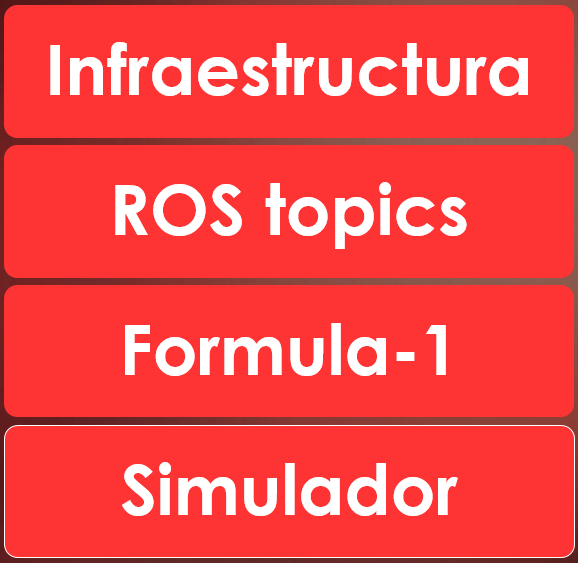
\includegraphics[width=0.4\linewidth, height=8cm]{figures/infraestructura_ch.png}
		\caption{Infraestructura del ejercicio Chrono}
		\label{fig.infraestructura_ch}
		\end{center}
\end{figure}

\subsection{Modelo de robot Formula-1}
El robot que se ha utilizado para esta práctica es un modelo de robot terrestre móvil que cuenta con 4 ruedas. El chasis elegido corresponde a un modelo de F1, específicamente del modelo RedBull. Además de este modelo se han incluido un amplio conjunto de modelos de F1 correspondientes a las principales escuderías que participan en la Fórmula 1. Esto supone un total de 12 modelos de coches de escuderías reales (India, HRT, Lotus, Mclaren, Mercedes, RedBull, Renault, Tororroso, Virgin y Williams) y un modelo sin marca comercial. Además, para cada modelo de coche ha sido necesario el desarrollo de dos modelos distintos, uno que incorpora una cámara, para esta práctica, y otro modelo que tiene un láser para otras prácticas de \textit{Robotics-Academy}. Gracias a estos modelos, en la práctica actual puede usarse indistintamente el modelo preferido por el estudiante (Figura \ref{fig.f1s}).

\begin{figure}[H]
  \begin{center}
    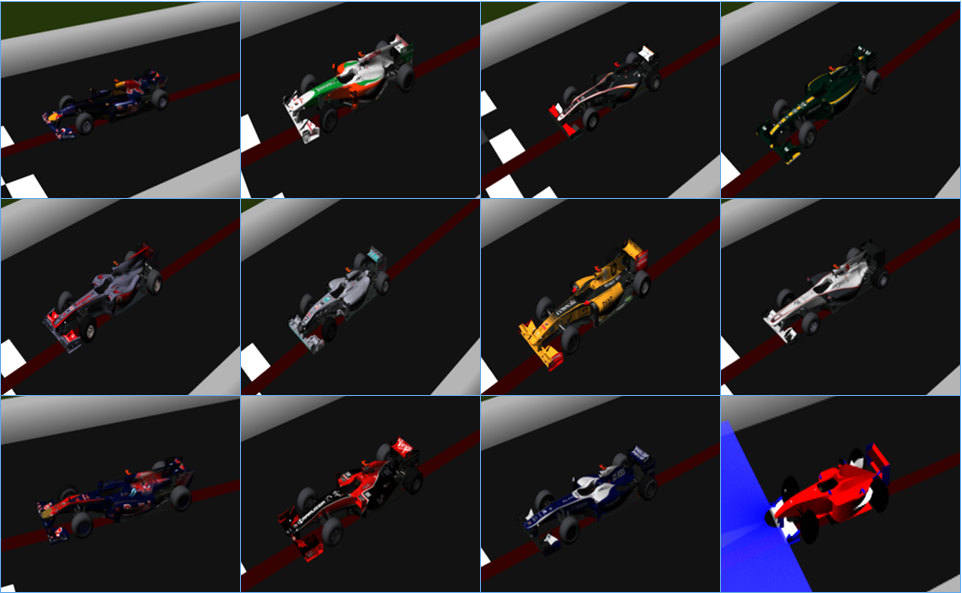
\includegraphics[width=0.99\linewidth, height=5.5cm]{figures/coches.png}
		\caption{Modelos disponibles de coches}
		\label{fig.f1s}
		\end{center}
\end{figure}

Tras crear el modelo, basta con importarlo en el mundo de Gazebo para su utilización.

\subsubsection{Cámara}
En la parte frontal del modelo se ha incluido una cámara para poder captar imágenes.
Los \textit{plugins} de la cámara dan soporte a una cámara conectada por USB con una velocidad de refresco de las imágenes de 20 fps. El tamaño de las imágenes, obtenidas periódicamente, es de 360x240 píxeles y están en formato crudo RGB. Gracias a esto, el modelo puede recoger imágenes a una velocidad suficiente y no perder de vista la línea. La velocidad de refresco de la cámara es un parámetro importante debido a que, dependiendo de este parámetro, entre otros, la velocidad del coche tendrá que adaptarse.

Las imágenes captadas por el \textit{plugin} son recogidas, por ejemplo, por el nodo ROS que, mediante un API sencillo, proporciona al estudiante las imágenes captadas y soporta la visualización de los filtros que se le apliquen a la imagen.

\subsubsection{Motor}
Para dotar al coche de movimiento, el modelo incluye un motor al que es posible conectarse, mediante un \textit{plugin}, y enviar órdenes para mover el coche. 
Con los \textit{topics} que ofrece ROS es posible enviar órdenes desde el nodo ROS al coche de manera sencilla con el HAL-API que proporciona al estudiante.

\subsubsection{Sensor de telemetría}
El sensor odométrico del modelo es imprescindible para esta práctica, ya que el nodo ROS recoge la odometría del robot y la publica en un mapa con el modelo del circuito. La odometría simulada utiliza la posición absoluta verdadera que maneja y actualiza el simulador de Gazebo para el coche.

Para representar la odometría, ROS utiliza \textit{quaternions}\footnote{\url{https://en.wikipedia.org/wiki/Quaternions_and_spatial_rotation}}. Se trata de una representación de la posición en 3D muy eficiente y numéricamente estable. Estos \textit{quaternions} se dividen en coordenadas ``x,y,z'' y orientación ``w''\footnote{\url{http://wiki.ros.org/tf2/Tutorials/Quaternions}}. Para las coordenadas x,y,z, ROS emplea la notación \textit{ENU}\footnote{\url{http://www.dirsig.org/docs/new/coordinates.html}}. Gracias a esta representación, el sensor de telemetría del coche almacena, progresivamente, \textit{quaternions} de la posición. 

\subsection{Escenario de Gazebo}
Para esta práctica se ha creado un modelo simulado del circuito de carreras Nürburgring (Alemania) acortado, llamado ``nurburgrinLineROS''. Mediante el uso de los softwares \textit{Blender} y \textit{SketchUp}, se ha modelado el circuito con una línea de salida, una grada, la carretera, paredes para evitar que el robot se salga del recorrido y césped de adorno (Figura 4.3).

\begin{figure}[H]
  \begin{center}
    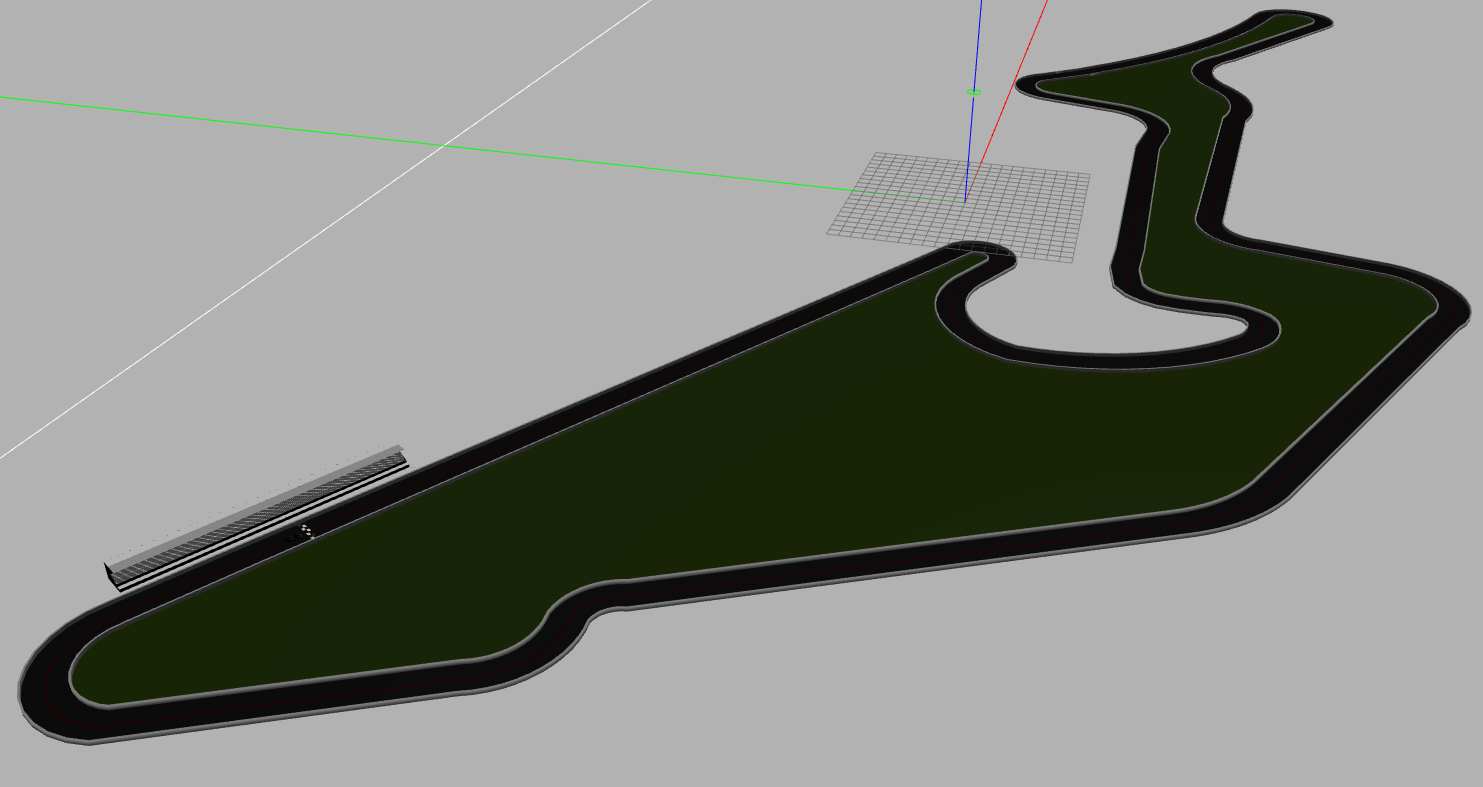
\includegraphics[width=0.95\textwidth, height=12cm]{figures/circuito.png}
		\caption{Modelo del circuito de Nürburging}
		\label{fig.circuito}
		\end{center}
\end{figure} 

\subsection{Ficheros de configuración} \label{sec.fichconf}
Para la incorporación a una simulación del modelo del circuito y del robot, es necesario la creación de un fichero de configuración que importe en \textit{Gazebo} los elementos de los que consta el escenario y su localización. Este fichero tiene la extensión \textit{.world} y \textit{Gazebo} es capaz de leerlo y mostrar el escenario al iniciarse.
El código del fichero creado para este ejercicio es el siguiente:

\lstset{language=XML, breaklines=true, basicstyle=\footnotesize}
\begin{lstlisting}[frame=single]
<?xml version="1.0"?>
<sdf version="1.4">
  <world name="default">
    <include>
      <uri>model://sun</uri>
    </include>
    <include>
      <uri>model://nurburgrinLine</uri>
      <pose>70 -47 0 0 0 0</pose>
    </include>
    <include>
      <uri>model://f1ROS</uri>
      <pose>0.05 -0.44 0 0 0 0.9</pose>
    </include>
  </world>
</sdf>
\end{lstlisting}

Además de este fichero de configuración, es necesario un fichero complementario que arranca los \textit{plugins y drivers} de ROS-Kinetic. Este archivo tiene la extensión \textit{.launch}. En él se pasan a \textit{Gazebo} argumentos como el nombre del fichero de configuración con el escenario, se establece el tiempo que se va a utilizar en el escenario, el posible lanzamiento de un GUI y otras opciones de depuración.
El fichero es el siguiente:

\lstset{language=XML, breaklines=true, basicstyle=\footnotesize}
\begin{lstlisting}[frame=single]
<?xml version="1.0" encoding="UTF-8"?>
<launch>
  <include file="$(find gazebo_ros)/launch/empty_world.launch">
    <arg name="world_name" value="nurburgrinLineROS.world"/>
    <arg name="paused" value="false"/>
    <arg name="use_sim_time" value="true"/>
    <arg name="gui" value="true"/>
    <arg name="headless" value="false"/>
    <arg name="debug" value="false"/>
    <arg name="verbose" default="false"/>
  </include>
</launch>
\end{lstlisting}

\section{Plantilla de nodo ROS}
Una vez explicada la infraestructura de la práctica, en esta sección se va a explicar la plantilla de nodo ROS desarrollada. Esta plantilla es una manera de ejecutar los ejercicios de \textit{Robotics-Academy} (Figura \ref{fig.na_ch}). Esta plantilla de nodo ROS de la práctica, está formada por:

\begin{itemize}
    \item Fichero principal.
    \item Fichero de solución
    \item GUI. Directorio con todos los ficheros para el funcionamiento del GUI.
\end{itemize}

El fichero principal es el código que va a ejecutarse al lanzar el nodo académico de la práctica. En él se especifican las conexiones con los \textit{topics} que se van a establecer, así como la inicialización del GUI.

En el fichero de solución hay un conjunto de funciones que aportan la funcionalidad de la práctica, como comenzar, parar, recoger imagen, así como las que desarrolle el alumno y el propio código con la solución de referencia.

\begin{figure}[H]
  \begin{center}
    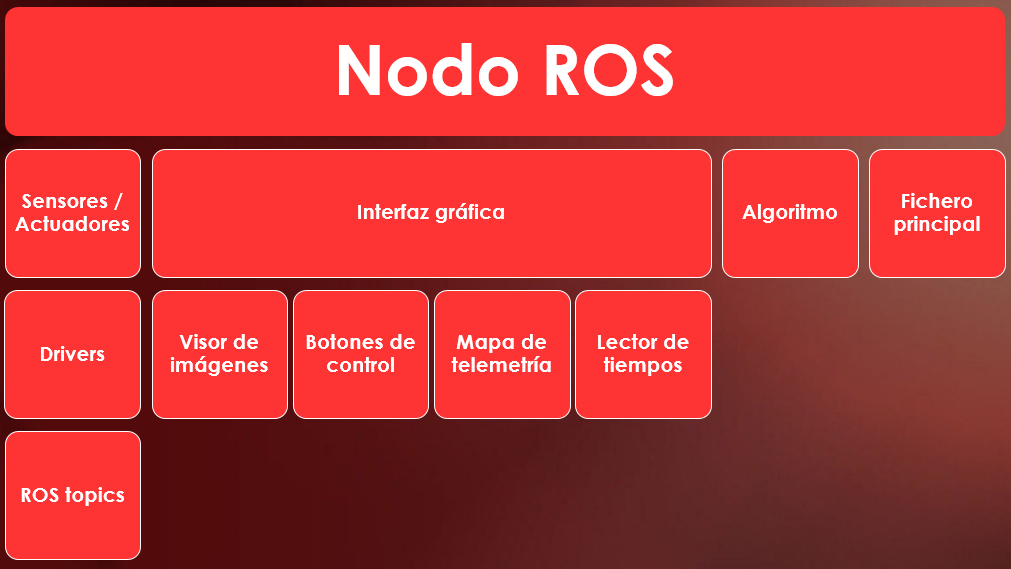
\includegraphics[width=0.9\textwidth, height=8cm]{figures/na_ch.png}
		\caption{Nodo Académico de Chrono}
		\label{fig.na_ch}
		\end{center}
\end{figure}

\subsection{Arquitectura software}
Este nodo ROS tiene dos hilos de ejecución, en lugar de uno monolítico, para aliviar la carga computacional. De esta manera se aumenta la velocidad a la que puede trabajar el simulador \textit{Gazebo} porque se aprovechan mejor los múltiples núcleos que puede tener el ordenador del estudiante.

\begin{itemize}
	\item Hilo de percepción y control: se encarga de la actualización de los datos de los sensores del robot. Este hilo se comunica con \textit{Gazebo} para recoger datos de la odometría y la cámara y para enviar las órdenes de control del motor con las que se mueve el robot. Además, ejecuta el código del estudiante, por lo que su carga computacional es bastante elevada.
	\item Hilo de la interfaz gráfica del usuario (GUI): se encarga del refresco del GUI de la práctica. En esta práctica tiene una carga computacional elevada dado que se encarga de refrescar las imágenes obtenidas por la cámara, un mapa del circuito con la posición actualizada del robot y del robot fantasma a vencer, y una lectura controlada de tiempos para sincronizar ambos coches.
\end{itemize}

Gracias a esta interfaz gráfica el estudiante puede servirse de algunos elementos de depuración que veremos en profundidad en la sección 5.3.2 y 5.3.3. De esta manera, solo tiene que centrarse en el desarrollo del algoritmo. El nodo académico dispone de una función reservada para que el alumno escriba su algoritmo en ella y pueda ver los resultados, todo ello viene indicado en las instrucciones, publicadas en el fichero \textit{README.md} de la práctica en el repositorio.

\subsection{Interfaz de sensores y actuadores}
Cualquiera de los modelos de Fórmula-1 creados utiliza los \textit{plugins} de ROS para dotar al modelo de movimiento, captación de imágenes y odometría. Estos \textit{plugins} son drivers de los sensores y actuadores del coche simulado, y permiten conectarse e intercambiar mensajes de ROS (\textit{topics}) con aplicaciones. Desde las aplicaciones son accesibles, de manera sencilla, usando dos bibliotecas:
\begin{itemize}
	\item \textit{libgazebo\_ros\_camera}
Para la captación de imágenes.
	\item \textit{libgazebo\_ros\_planar\_move}
Para el control del motor y obtener la odometría.
\end{itemize}

Tanto para recoger los datos de los sensores como para enviar los datos de los actuadores, el nodo ROS proporciona un HAL-API de interconexión con los \textit{topics}. De esta manera, es sobre esta interfaz sobre la que el alumno debe apoyarse para desarrollar su algoritmo, dejando los detalles de más bajo nivel, como la procedencia de los sensores o la conexión con el coche simulado, transparentes para el mismo. EL HAL-API proporcionado por este nodo ROS es el siguiente:

\begin{itemize}
	\item \textit{self.pose3d.getPose3d()}: con esta función se obtienen los datos de odometría y posición del coche. Se conecta con la biblioteca \textit{libgazebo\_ros\_planar\_move}.
	\item \textit{self.camera.getImage()}: con esta función se recogen las imágenes obtenidas por la cámara. Se conecta con la biblioteca \textit{libgazebo\_ros\_camera}.
	\item \textit{self.motors.senV() o self.motors.sendW()}: con esta función se ordena las velocidades de avance y giro. Se conecta con la biblioteca \textit{libgazebo\_ros\_planar\_move}.
\end{itemize}

\subsection{Interfaz gráfica}
La interfaz gráfica del usuario (GUI) se utiliza para representar información relacionada con los sensores del robot. Además, permite teleoperar el robot y lanzar/detener la ejecución del algoritmo programado por el estudiante. Esto es muy útil para la depuración, ya que permite la visualización de las órdenes que genera el algoritmo al robot y comprobar su movimiento.

Esta GUI (Figura \ref{fig.guich}) está formada por cuatro \textit{widgets}, uno para el visionado del robot, otro para su comportamiento, otro para su odometría y otro para la sincronización de la grabación del coche récord.


\begin{figure}[H]
  \begin{center}
    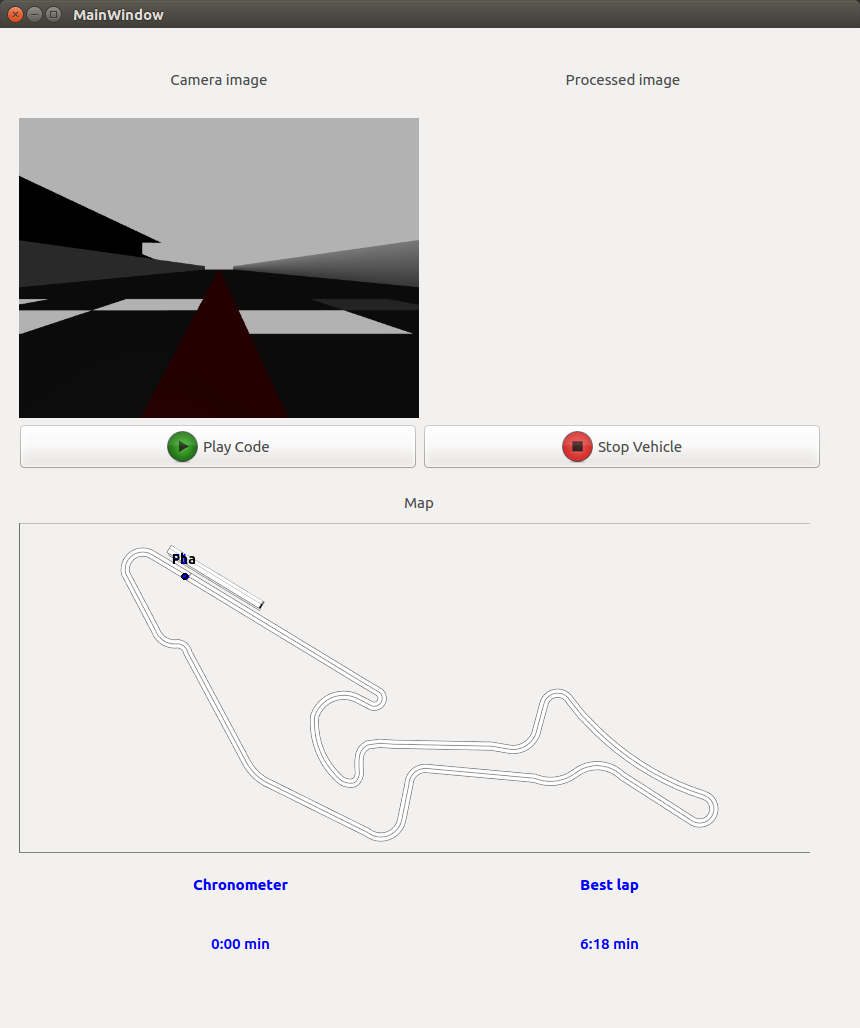
\includegraphics[width=.75\textwidth]{figures/GUI_Chrono.png}
		\caption{Interfaz Gráfica Chrono}
		\label{fig.guich}
		\end{center}
\end{figure}

En el \textit{widget} superior se pueden visualizar las imágenes captadas por la cámara que incorpora el robot. Gracias a ella, el alumno puede tener una idea de la visión del robot y programar una solución de una manera más sencilla. A la derecha de la ventana del visor de imágenes de la cámara, se ha incluido otra ventana de visualización. Esta ventana se encarga de mostrar el procesamiento de la imagen desarrollado por el alumno. Gracias a esta ventana, el alumno puede hacerse una idea del algoritmo de procesamiento de imagen que ha desarrollado (Figura \ref{fig.vich}).

\begin{figure}[H]
  \begin{center}
    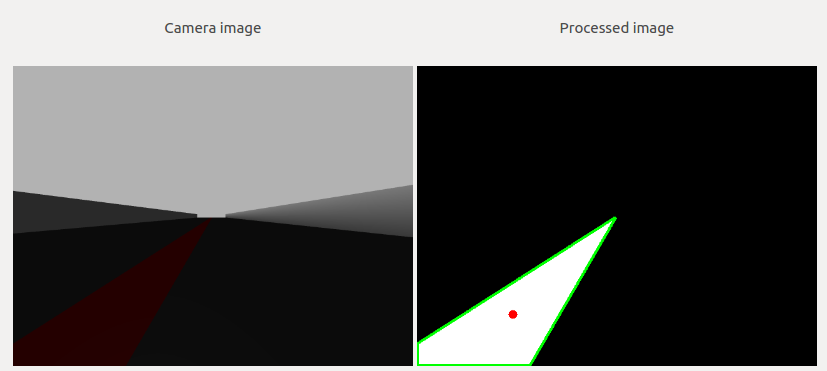
\includegraphics[width=0.98\textwidth]{figures/visor_imagen_chrono.png}
		\caption{Visor de imágenes de Chrono}
		\label{fig.vich}
		\end{center}
\end{figure}

El segundo \textit{widget} está formado por un mapa del circuito, en este caso el circuito de Nürburgring, en el que se pueden visualizar las posiciones instantáneas del robot y del robot fantasma con el récord del circuito.

Además de estos \textit{widget}, en el GUI se incluyen distintos botones de control para hacer una pausa en la ejecución del algoritmo y para reiniciar la posición del teleoperador. El primer botón se llama \textit{pushButton} y consiste en un botón interactivo para iniciar el código programado por el alumno y para parar el código (Figura \ref{fig.bpch} y \ref{fig.bsch}). Esta pause que introduce implica la detención de la ejecución del código enviando, de manera recursiva, la orden de mantener la posición actual. El segundo botón se llama \textit{ResetButton} y se utiliza para reiniciar el teleoperador de la interfaz gráfica y hacer que el robot no se mueva.

\begin{figure}[H]
	\begin{center}
	    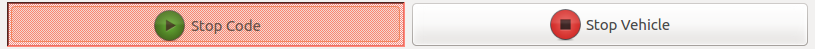
\includegraphics[width=0.98\textwidth]{figures/boton_pausa_chrono.png}
		\caption{Botón de pausa de la ejecución del código del estudiante}
		\label{fig.bpch}
	\end{center}
\end{figure}
\begin{figure}[H]
	\begin{center}
        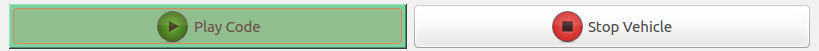
\includegraphics[width=0.98\textwidth]{figures/boton_start_chrono.png}
		\captionof{figure}{Botón de comienzo de la ejecución del código del estudiante}
		\label{fig.bsch}
	\end{center}
\end{figure}

La parte inferior del GUI tiene un lector de tiempos en el que se muestra el tiempo simulado de \textit{Gazebo} y, por lo tanto, el tiempo que está necesitando el robot para completar la vuelta. A su derecha se muestra el tiempo del récord del circuito para que el alumno tenga una idea de la optimización que necesita el código de control de movimiento del robot para que sea más eficiente.

\subsubsection{Coche de referencia}
El nodo ROS, concretamente el hilo de ejecución encargado del interfaz gráfico (GUI), se encarga de cargar la imagen del mapa en el GUI. Una vez hecho esto, recoge los datos de odometría del sensor \textit{Pose3D} y dibuja su posición en el mapa. Adicionalmente, recoge los datos de odometría del fichero de grabación de ROS para extraer la posición del coche fantasma de referencia y la dibuja en el mapa también.

\begin{figure}[H]
  \begin{center}
    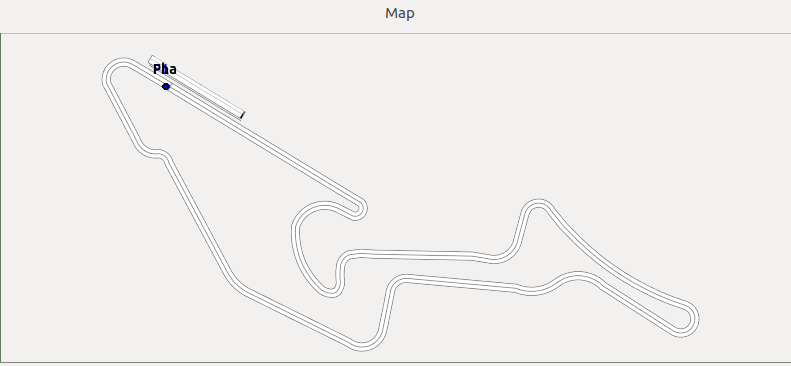
\includegraphics[width=0.98\textwidth]{figures/mapa_chrono.png}
		\caption{Mapa del GUI}
		\label{fig.mapach}
		\end{center}
\end{figure}

Esta ejecución es bastante pesada computacionalmente, dado que requiere de una actualización constante para reflejar una posición lo más exacta posible, tanto del coche fantasma como del coche programado por el estudiante. Es por ello que se utiliza el hilo de ejecución proporcionado por el GUI, en lugar del hilo de percepción y control. Esto alivia a la ejecución principal de una gran carga computacional.

Este ha sido el principal reto de esta práctica por su complejidad a la hora de recoger los datos, tanto de \textit{Gazebo}, como de \textit{ROSbag} y sincronizarlos. El problema que se planteaba en la sincronización de tiempos era el hecho de que los tiempos de \textit{Gazebo} en vivo se sincronizan mediante el tiempo de simulación del propio simulador, pero los tiempos grabados mediante ROSbag, se reproducen mediante el tiempo real. Esto supone una desincronización muy grande ya que, en el ordenador de trabajo, el tiempo de simulación era aproximadamente un 0,15 veces el tiempo real. Adicionalmente existe el problema de que el tiempo de simulación depende de la potencia de cómputo de cada ordenador, por lo que el ajuste entre los ritmos de reproducción no se puede realizar con una constante porque sería un hándicap muy grande para los ordenadores potentes, que se verían afectados a reproducir de una manera muy lenta.

En este aspecto, debían abordarse los dos problemas propuestos de manera simultánea. Por un lado, sincronizar el tiempo de reproducción con el tiempo de simulación, y por otro llevar un ritmo del tiempo de simulación adaptado para la carga de cómputo que pueda soportar cada ordenador. Adicionalmente se encontró un problema adicional con la reproducción de la grabación de ROSbag: las etiquetas de tiempo de las que consta no se inicializan desde el comienzo, sino que se graban con el tiempo simulado actual. Es por esto que la reproducción comienza con una etiqueta temporal distinta de cero.

Para solucionar todos estos problemas ha sido necesaria la definición de varios conceptos:

\begin{itemize}
	\item \textit{Tiempo de grabación}: este tiempo representa el ritmo al que se reproduce la grabación de ROSbag.
	\item \textit{Tiempo simulado}: este tiempo representa el tiempo al que se refresca el simulador \textit{Gazebo}.
	\item \textit{Tiempo de reproducción}: este tiempo se basa en el tiempo de simulación pero restándole el offset del comienzo de la práctica. Por ello empieza cuando el estudiante ejecuta la práctica en lugar de cuando se inicia el simulador.
\end{itemize}

El algoritmo de simulación comienza recogiendo el instante de tiempo en el que el alumno ejecuta su código mediante el comando:

\lstset{language=Python, breaklines=true, basicstyle=\footnotesize}
\begin{lstlisting}[frame=single]
initime = rospy.Time.from_sec(rospy.get_time()).to_sec()
\end{lstlisting}

Una vez obtenido el tiempo inicial, es necesario recoger el instante de tiempo en el que estamos refrescando la sincronización:

\lstset{language=Python, breaklines=true, basicstyle=\footnotesize}
\begin{lstlisting}[frame=single]
sim_time = rospy.Time.from_sec(rospy.get_time()).to_sec()
\end{lstlisting}

Además de estos dos tiempos, es necesario conocer el tiempo de la primera etiqueta de la grabación de ROSbag para comenzar a leer las etiquetas desde ese offset:
\lstset{language=Python, breaklines=true, basicstyle=\footnotesize}
\begin{lstlisting}[frame=single]
rep_start = str(bag).split('start:       ')[1].split(' ')[4].split()[0][1:-1]
\end{lstlisting}
Con el tiempo de simulación actual, el tiempo inicial y el tiempo de inicio de la reproducción, podemos obtener el tiempo con el que vamos a comparar las etiquetas temporales de la grabación para saber si tenemos que leer la etiqueta temporal y actualizar la posición del coche fantasma en el mapa del GUI o seguir devolviendo la misma posición porque es pronto.

\lstset{language=Python, breaklines=true, basicstyle=\footnotesize}
\begin{lstlisting}[frame=single]
t_sim_unif = sim_time - initime + float(rep_start)
\end{lstlisting}

Gracias a esta sincronización se pueden devolver los valores de telemetría grabados para la solución con el récord de la vuelta para el coche fantasma y actualizar su posición en el mapa. A continuación, se describe el código utilizado para la sincronización:

\lstset{language=Python, breaklines=true, basicstyle=\footnotesize}
\begin{lstlisting}[frame=single]
def synchronize(self):
        global posx, posy, cursor

        t_sim_unif = sim_time - initime + float(rep_start)
        if initime != 0.0 and t_sim_unif != 0.0:
            for (topic,msg,t) in bag.read_messages(start_time=rospy.Time(t_sim_unif-0.05)):
                t = t.to_sec()
                if t_sim_unif > t:
                    try:
                        posx = str(msg).split('x: ')[1].split()[0]
                        posy = str(msg).split('y: ')[1].split()[0]
                        return float(posx), float(posy)
                    except IndexError:
                        pass
                else:
                    return float(posx), float(posy)

        else:
            return float(posx), float(posy)
\end{lstlisting}

en la Figura \ref{fig.ltch} se muestra el \textit{widget} en el GUI con la práctica iniciada. A la izquierda se puede visualizar el chronómetro con la duración de la ejecución y a su derecha se encuentra el registra con la duración de la vuelta para la grabación que se esté reproduciendo.

\begin{figure}[H]
  \begin{center}
    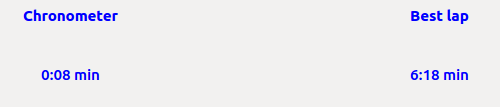
\includegraphics[width=0.98\textwidth]{figures/lector_tiempos_chrono.png}
		\caption{Lector de tiempos de Chrono}
		\label{fig.ltch}
		\end{center}
\end{figure}

\section{Solución de referencia}
La solución desarrollada ha sido creada por completo utilizando la librería \textit{OpenCV}, con funciones \textit{Built-in} proporcionadas por la misma que facilitan la comprensión del código programado. Gracias a esto, la velocidad del robot es mayor y, por consiguiente, completa la vuelta al circuito sin colisiones y en un tiempo menor que la solución previamente existente para el ejercicio ``sigue-líneas'' en \textit{Robotics-Academy}.

\subsection{Procesamiento de imagen} \label{sec.pdi}
El procesamiento de la imagen captada por la cámara, comienza con la recogida de la imagen guardada en el búffer de la misma con la instrucción:

\lstset{language=Python, breaklines=true, basicstyle=\footnotesize}
\begin{lstlisting}[frame=single]
input_image = self.camera.getImage().data
\end{lstlisting}

Gracias a esta instrucción es posible ver la imagen captada en la interfaz gráfica del usuario.

Una vez obtenida la imagen, hay que transformarla a una imagen HSV\footnote{\url{https://es.wikipedia.org/wiki/Modelo_de_color_HSV}} para poder seleccionar el color rojo de la línea central del circuito:

\lstset{language=Python, breaklines=true, basicstyle=\footnotesize}
\begin{lstlisting}[frame=single]
image_HSV = cv2.cvtColor(input_image, cv2.COLOR_RGB2HSV)
\end{lstlisting}

Tras obtener la imagen HSV, podemos seleccionar el rango de valores que componen el rojo de la línea como un array con la intensidad mínima y máxima del color.

\lstset{language=Python, breaklines=true, basicstyle=\footnotesize}
\begin{lstlisting}[frame=single]
value_min_HSV = np.array([0, 150, 0])
value_max_HSV = np.array([180, 255, 255])
\end{lstlisting}

Con esos valores realizamos un filtrado de la imagen para obtener la línea roja exclusivamente:

\lstset{language=Python, breaklines=true, basicstyle=\footnotesize}
\begin{lstlisting}[frame=single]
image_HSV_filtered = cv2.inRange(image_HSV, value_min_HSV, value_max_HSV)
\end{lstlisting}

Usamos el filtro obtenido como una máscara para filtrar la imagen y obtener de esta forma la imagen filtrada en blanco y negro. El blanco serán los colores que pasen el filtro y en negro obtendremos el resto de colores. En este caso, obtendremos la línea roja del circuito en color blanco y el resto de la imagen en negro (Figura \ref{fig.vich2}):

\lstset{language=Python, breaklines=true, basicstyle=\footnotesize}
\begin{lstlisting}[frame=single]
image_HSV_filtered_Mask = np.dstack((image_HSV_filtered, image_HSV_filtered, image_HSV_filtered))
\end{lstlisting}

\begin{figure}[H]
  \begin{center}
    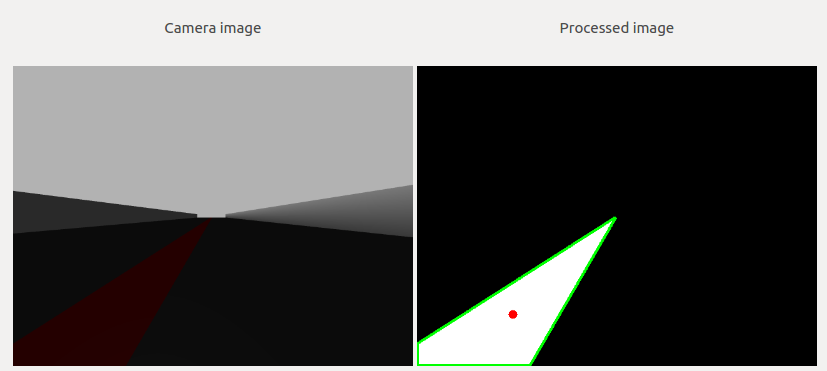
\includegraphics[width=0.98\textwidth]{figures/visor_imagen_chrono.png}
		\caption{Visor de imágenes de Chrono}
		\label{fig.vich2}
		\end{center}
\end{figure}

Una vez filtrada la imagen, se obtienen los contornos de la zona filtrada. Para ello, es necesario convertir la imagen a escala de grises:

\lstset{language=Python, breaklines=true, basicstyle=\footnotesize}
\begin{lstlisting}[frame=single]
imgray = cv2.cvtColor(image_HSV_filtered_Mask, cv2.COLOR_BGR2GRAY)
\end{lstlisting}

De esta manera, se pueden conseguir los píxeles que tiene un contraste mayor con sus vecinos, obteniendo el contorno:

\lstset{language=Python, breaklines=true, basicstyle=\footnotesize}
\begin{lstlisting}[frame=single]
ret, thresh = cv2.threshold(imgray, 127, 255, 0)
_, contours, hierarchy = cv2.findContours(thresh, cv2.RETR_TREE, cv2.CHAIN_APPROX_SIMPLE)
\end{lstlisting}

Una vez conseguido el contorno, se dibuja en la imagen filtrada:

\lstset{language=Python, breaklines=true, basicstyle=\footnotesize}
\begin{lstlisting}[frame=single]
cv2.drawContours(image_HSV_filtered_Mask, contours, -1, (0,255,0), 3)
\end{lstlisting}

El siguiente paso es robustecer el código en el caso de que en el filtrado de la imagen se detecten dos zonas con filtro. Esto se puede producir cuando hay una curva y, debido a la resolución de la cámara, recoge la línea roja pero incompleta. Esto produce lagunas de filtro de color en las que no se visualiza la línea por completo, sino cortada. Para evitar un fallo en el algoritmo ha sido necesaria la inclusión código que recoge todas las zonas filtradas y selecciona la de mayor área:

\lstset{language=Python, breaklines=true, basicstyle=\footnotesize}
\begin{lstlisting}[frame=single]
area = []
for pic, contour in enumerate(contours):
    area.append(cv2.contourArea(contour))
if len(area) > 1:
    if area[0] < area[1]:
        M = cv2.moments(contours[1])
    else:
        M = cv2.moments(contours[0])
else:
    M = cv2.moments(contours[0])
\end{lstlisting}

Esta solución no necesita comprobar la imagen completa píxel a píxel, sino que filtra el área de la línea y procesa su centro. Se obtienen los valores de los ejes x e y de la zona filtrada, que forman el centro del área que ha sido filtrada:

\lstset{language=Python, breaklines=true, basicstyle=\footnotesize}
\begin{lstlisting}[frame=single]
if int(M['m00']) != 0:
    self.cx = int(M['m10']/M['m00'])
    self.cy = int(M['m01']/M['m00'])
\end{lstlisting}

Gracias a estos valores, en concreto al valor del eje x, podemos saber la diferencia de posición que tiene el robot con el centro de la línea roja, es decir, la diferencia de posición del robot con el centro del circuito. Para facilitar este cálculo se ha dibujado un punto en la imagen filtrada con los valores del eje y el eje y para que sea visualizado:

\lstset{language=Python, breaklines=true, basicstyle=\footnotesize}
\begin{lstlisting}[frame=single]
cv2.circle(image_HSV_filtered_Mask, (self.cx, self.cy), 7, np.array([255, 0, 0]), -1)
\end{lstlisting}

Para la visualización de la imagen procesada, basta con utilizar la instrucción proporcionada por la interfaz gráfica del usuario:

\lstset{language=Python, breaklines=true, basicstyle=\footnotesize}
\begin{lstlisting}[frame=single]
self.setImageFiltered(image_HSV_filtered_Mask)
\end{lstlisting}

\subsection{Control de movimiento}
Una vez hecho el filtro de color y contornos, el control de movimiento es sencillo, pues basta con obtener el valor del eje x cuando el coche está alineado con la línea recta y tomarlo como el movimiento nulo. Tras esto, se puede definir el giro del robot en consonancia con este valor de movimiento nulo.

En función de la distancia que tenga el coche con el centro del filtrado, se define un control de velocidad de avance y de giro. El control de la velocidad de avance varía en casos extremos en los que la distancia es grande, para dar tiempo a la velocidad de giro a corregir la posición del coche. El control de velocidad de giro se realiza de manera iterativa en función esta distancia, para ello se define un valor para compararlo con la desviación actual. 

\lstset{language=Python, breaklines=true, basicstyle=\footnotesize}
\begin{lstlisting}[frame=single]
if self.cx < 50:
    self.motors.sendV(1.5)
else:
    self.motors.sendV(3.5)

self.motors.sendW((153-int(self.cx))*0.01)
\end{lstlisting}

\section{Validación experimental}
La optimización de los algoritmos anteriores ha sido posible gracias a la realización de diversos experimentos. Estos experimentos han hecho salir a la luz errores en el algoritmo desarrollado que han sido subsanados.

Además, se han realizado experimentos globales donde se ha validadp la práctica en su totalidad, nodo académico, infraestructura de la práctica y solución desarrollada.

\subsection{Ejecución típica}
Se ha preparado un documento \textit{README.md}, incluido en la infraestructura de la práctica, que sirve de guía al alumno a la hora de ejecutar la práctica. En él se incluye información acerca de su ejecución, la API de los sensores y actuadores de ROS e, incluso, un vídeo demostrativo con una ejecución.

Para ejecutar la práctica es necesario lanzar en una terminal el fichero de configuración de ROS, llamado \textit{f1-chrono.launch}, descrito en la sección \ref{sec.fichconf}. Para lanzar el fichero hay que ejecutar el siguiente comando:

\lstset{language=bash, breaklines=true, basicstyle=\footnotesize}
\begin{lstlisting}[frame=single]
roslaunch f1-chrono.launch
\end{lstlisting}

Una vez lanzado el comando en la terminal, se abrirá el simulador \textit{Gazebo} con el escenario del circuito (Figura \ref{fig.circuito}).

\begin{figure}[H]
  \begin{center}
    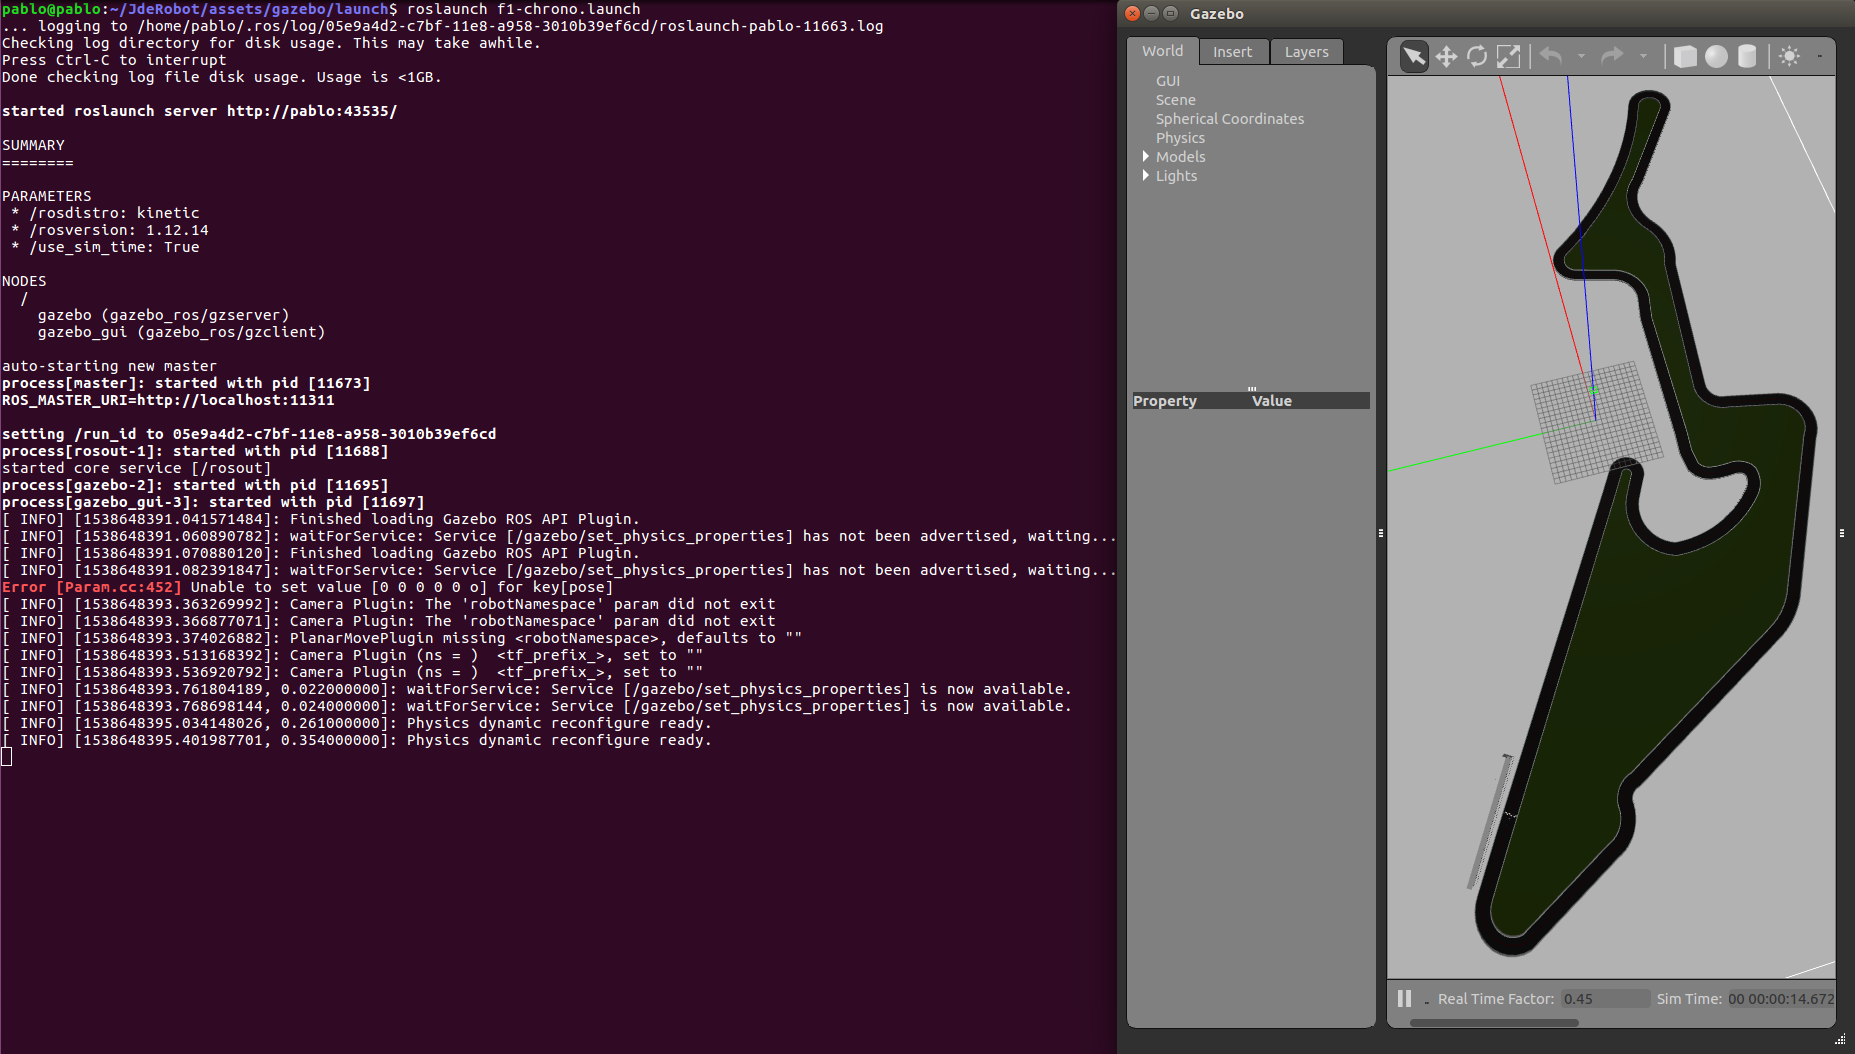
\includegraphics[width=0.98\textwidth]{figures/roslaunch_chrono.png}
		\caption{Inicialización ROS y Gazebo}
		\label{fig.roslaunchch}
		\end{center}
\end{figure}

Para iniciar el nodo ROS, será necesario ejecutar otro comando en una terminal distinta:

\lstset{language=bash, breaklines=true, basicstyle=\footnotesize}
\begin{lstlisting}[frame=single]
cd ~/Academy/exercises/chrono
python2 chrono.py
\end{lstlisting}

Una vez ejecutado el comando, el nodo ROS enlazará los sensores y actuadores proporcionados por \textit{ROS-Kinetic} mediante el fichero de configuración lanzado previamente a las variables:

\begin{itemize}
    \item self.camera
    \item self.pose3d
    \item self.motors
\end{itemize}

Con estas variables, el nodo ROS se comunica con los \textit{drivers} de \textit{ROS-Kinetic}.
Además de realizar la conexión con los sensores y actuadores, al ejecutar la instrucción, nos aparecerá la interfaz gráfica de usuario (GUI) en la que se podrá visualizar las imágenes recogidas por la cámara, los botones de control, el mapa del circuito y el lector de tiempos (Figura \ref{fig.inaGch}).

\begin{figure}[H]
  \begin{center}
    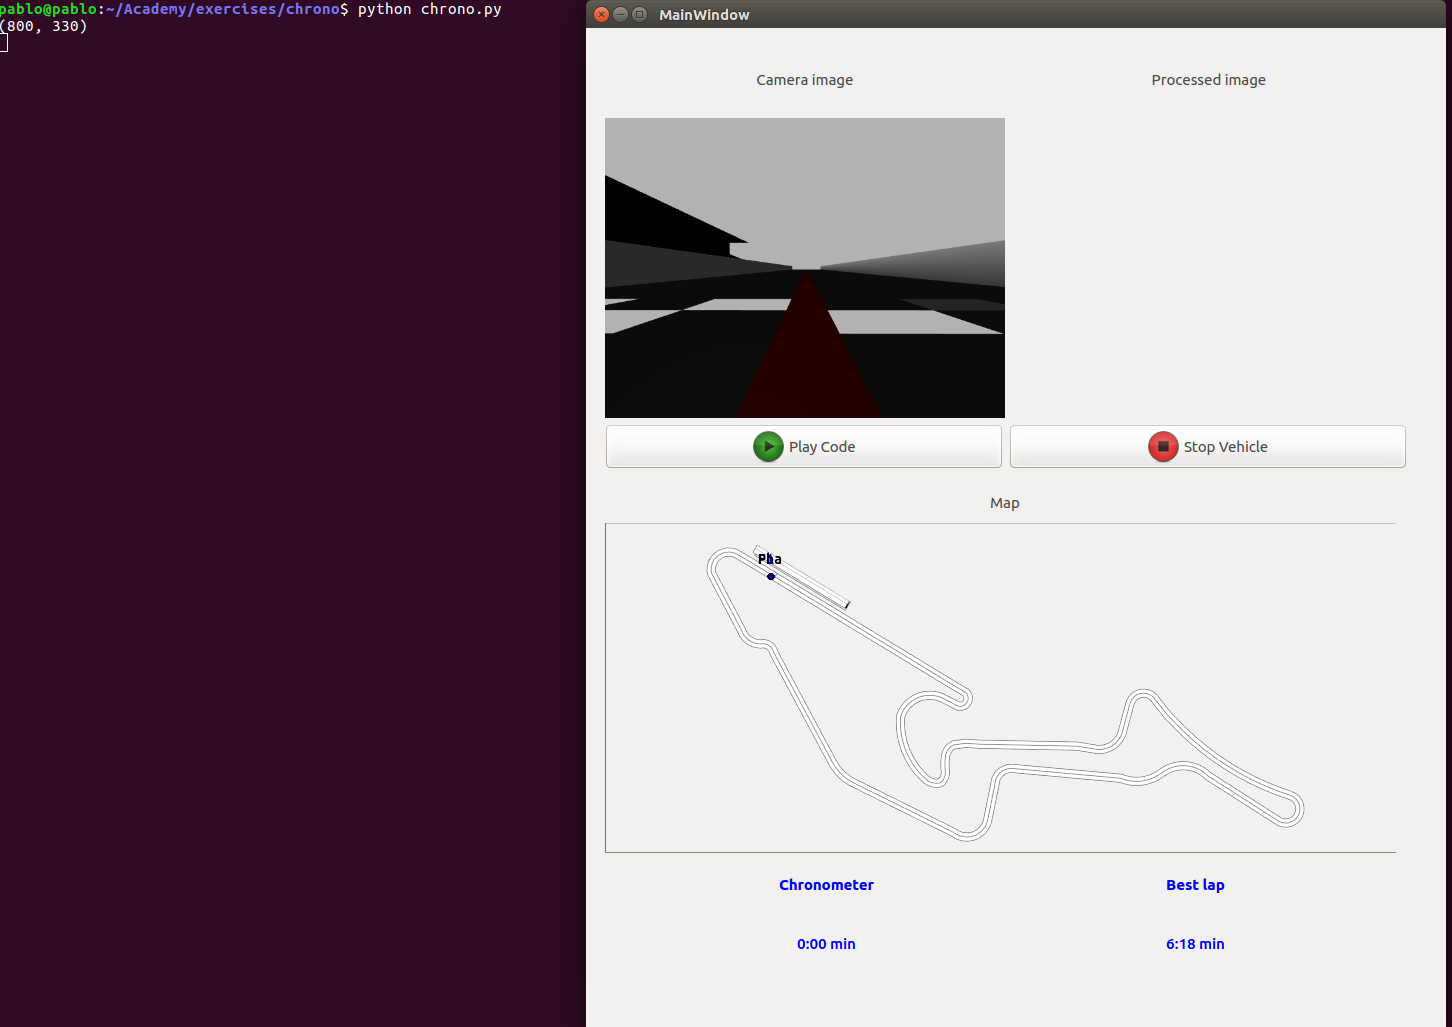
\includegraphics[width=0.98\textwidth]{figures/init_na_chrono.png}
		\caption{Inicialización del nodo académico y el GUI}
		\label{fig.inaGch}
		\end{center}
\end{figure}

Una vez inicializados los \textit{drivers de ROS-Kinetic}, el escenario en el simulador y el nodo académico, con su GUI, se puede iniciar el algoritmo desarrollado por el alumno pulsando sobre el botón ``Play Code''. De esta manera, los resultados de la lógica programada podrán ser visualizados tanto en el GUI, como en el simulador.
 
\subsection{Ejecución en movimiento}
Una vez conseguido un algoritmo que procese las imágenes en movimiento con el teleoperador, el alumno puede pasar a la última fase del desarrollo de la solución, el control de movimiento del robot. Para ello deberá utilizar el procesamiento de la imagen realizado en la primera parte del desarrollo del algoritmo para poder dotar al robot de un movimiento en función del filtrado que realice de la línea roja del circuito.

En este punto hay que tener especial cuidado con las curvas dado que la línea varía bruscamente y, con una velocidad elevada, la línea puede salirse del rango de captura de imagen de la cámara y, por lo tanto, el algoritmo producirá un error (a menos que se programe una solución para ese caso). Es por esto que el alumno debe ser consciente de la velocidad de refresco de la imagen de la cámara, 20 fotogramas por segundo, y de la velocidad con la que el nodo ROS recoge las imágenes de la cámara. La velocidad de refresco del GUI es la limitante debido a la carga computacional que tiene la hebra de la interfaz gráfica. Debido a la odometría y a la sincronización, el hilo de ejecución no recoge las 20 imágenes por segundo que capta la cámara, sino que dependerá de la potencia computacional de cada ordenador.

\begin{figure}[H]
  \begin{center}
    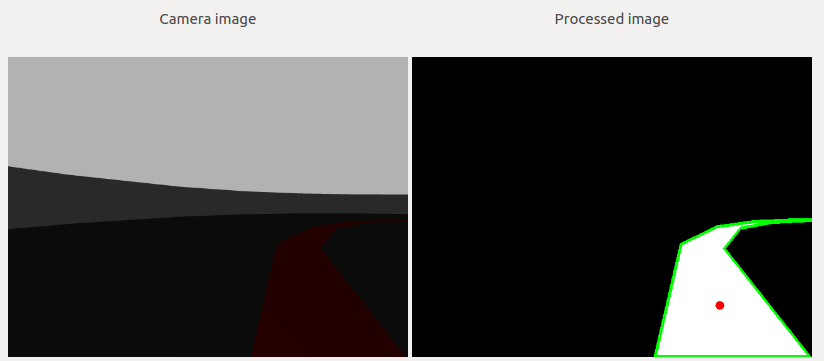
\includegraphics[width=0.98\textwidth]{figures/filtrado_curvas_chrono.png}
		\caption{Ejemplo de procesamiento de la imagen en las curvas}
		\label{fig.pdiecch}
		\end{center}
\end{figure}

Por último, una vez que se ha desarrollado el algoritmo completo, se puede ejecutar la práctica con el algoritmo (vídeo demostrativo de YouTube: \url{https://www.youtube.com/watch?v=OyUqYTKZHmU}).

\begin{figure}[H]
  \begin{center}
    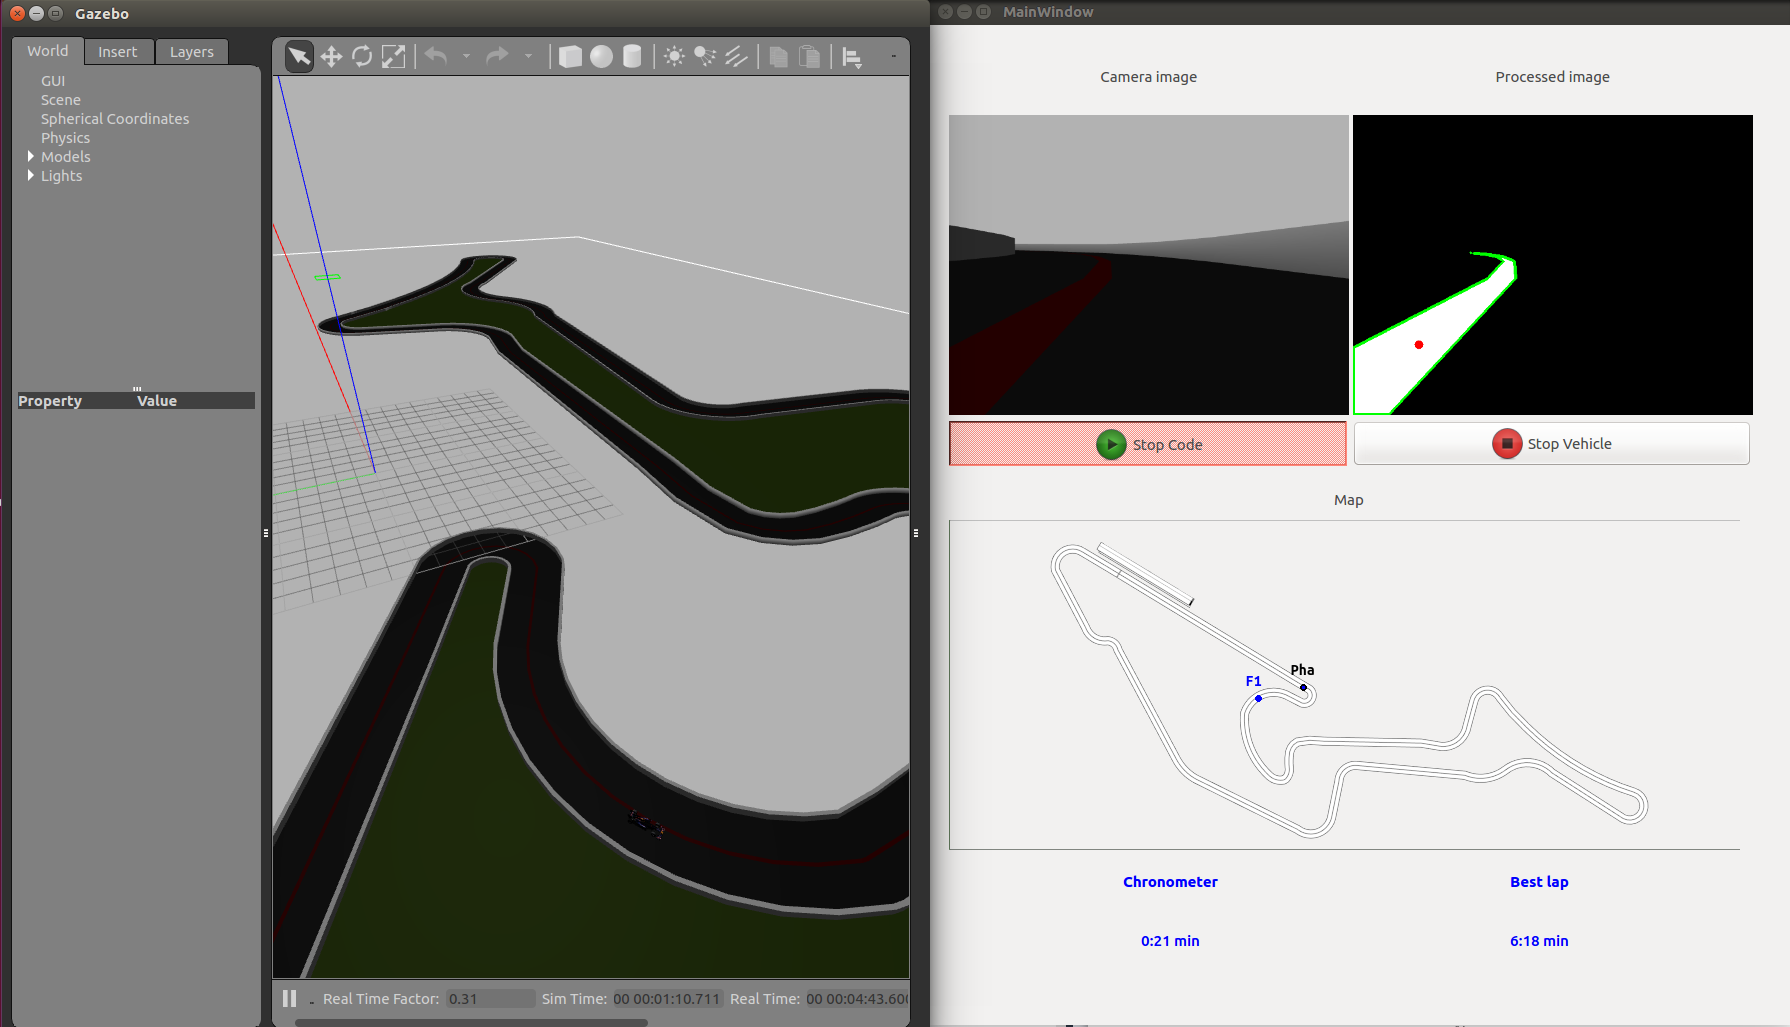
\includegraphics[width=0.98\textwidth]{figures/ejec_algoritmo_ch.png}
		\caption{Ejecución con la solución}
		\label{fig.ealgch}
		\end{center}
\end{figure}

En el caso en el que el alumno no programe el control de movimiento en su algoritmo, es posible ejecutar el código perceptivo de igual manera. Esto es útil para depurar el algoritmo de procesamiento de imagen. 

El alumno tiene dos opciones en este aspecto. La primera consiste en dejar el robot inmóvil y ver el procesamiento realizado en la ventana para la imagen procesada del GUI. 

Otra opción, una vez haya superado esa primera prueba, es seleccionar una velocidad fija para mover el robot y visualizar el filtrado en movimiento.
Con esta ejecución semi-móvil de la práctica, el alumno también puede visualizar, no solo la telemetría del fantasma, que se visualizará cada vez que se ejecute el algoritmo, sino la telemetría del robot a programar. Con esto, el alumno se puede hacer una idea de la velocidad a la que tiene que programar el control de movimiento para ser más veloz que el récord del circuito.

\section{Cuadernillo académico Jupyter}
Como parte paralela a la práctica incluida en \textit{Robotics-Academy}, se ha desarrollado otra plantilla paralela, con cuadernillos de \textit{Jupyter} en lugar de nodo ROS. Gracias a esto el alumno puede programar y ejecutar el código mediante la utilización del navegador web que prefiera.

Esto supone un paso importante hacia la multiplataforma del entorno docente \textit{Robotics-Academy}, dado que el alumno puede acceder a las prácticas desde el sistema operativo que prefiera, sólo necesita acceso a internet.

Ha sido necesaria una reestructuración del nodo ROS y de los ficheros que lo componen, además del método para el desarrollo del algoritmo. Se ha eliminado el GUI del nodo ROS y se han introducido los hilos de percepción y control en el cuadernillo de Jupyter. De esta manera, el alumno sólo debe rellenar una celda del cuadernillo con el algoritmo desarrollado.

\begin{figure}[H]
  \begin{center}
    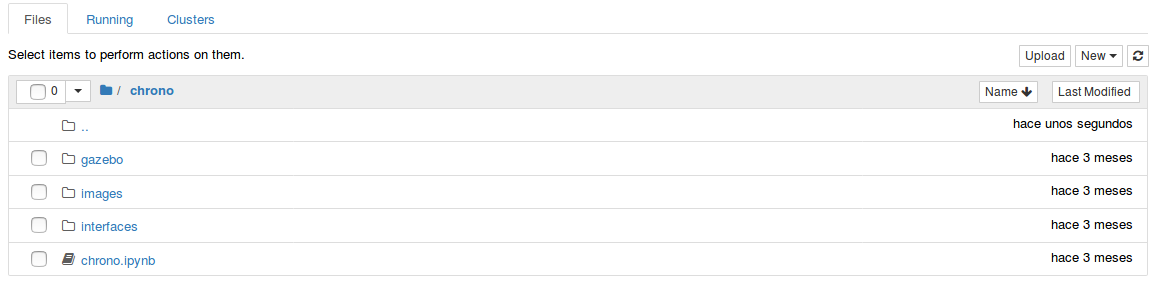
\includegraphics[width=0.98\textwidth]{figures/estructura_jupyter.png}
		\caption{Estructura de la práctica en Jupyter}
		\label{fig.ejch}
		\end{center}
\end{figure}

La plantilla de Jupyter tiene la estructura de la Figura \ref{fig.ejch}. Como puede verse es diferente a la estructura presente en el nodo ROS de \textit{Robotics-Academy}. Ahora se divide en los siguiente ficheros y carpetas:

\begin{itemize}
    \item images: en este directorio aparecen las imágenes contenidas en el cuadernillo.
    \item gazebo: en este directorio está el fichero de configuración con el escenario y con los \textit{drivers} de \textit{ROS-Kinetic}.
    \item interfaces: en este directorio se encuentran los \textit{drivers}.
    \item chrono.ipynb: este fichero es el cuadernillo ejecutable en Jupyter.
\end{itemize}

Para acceder a la práctica, el alumno debe iniciar Jupyter introduciendo en la terminal el siguiente comando:

\lstset{language=bash, breaklines=true, basicstyle=\footnotesize}
\begin{lstlisting}[frame=single]
cd ~/Jupyter
jupyter-notebook
\end{lstlisting}

Con esto se abrirá el navegador web por defecto en la carpeta local Jupyter. Una vez hecho esto, navegaremos hacia el directorio de la práctica de Jupyter ``Chrono'' y abriremos el fichero ``Chrono.ipynb''. Tras esto se mostrará la siguiente imagen del cuadernillo:

\begin{figure}[H]
  \begin{center}
    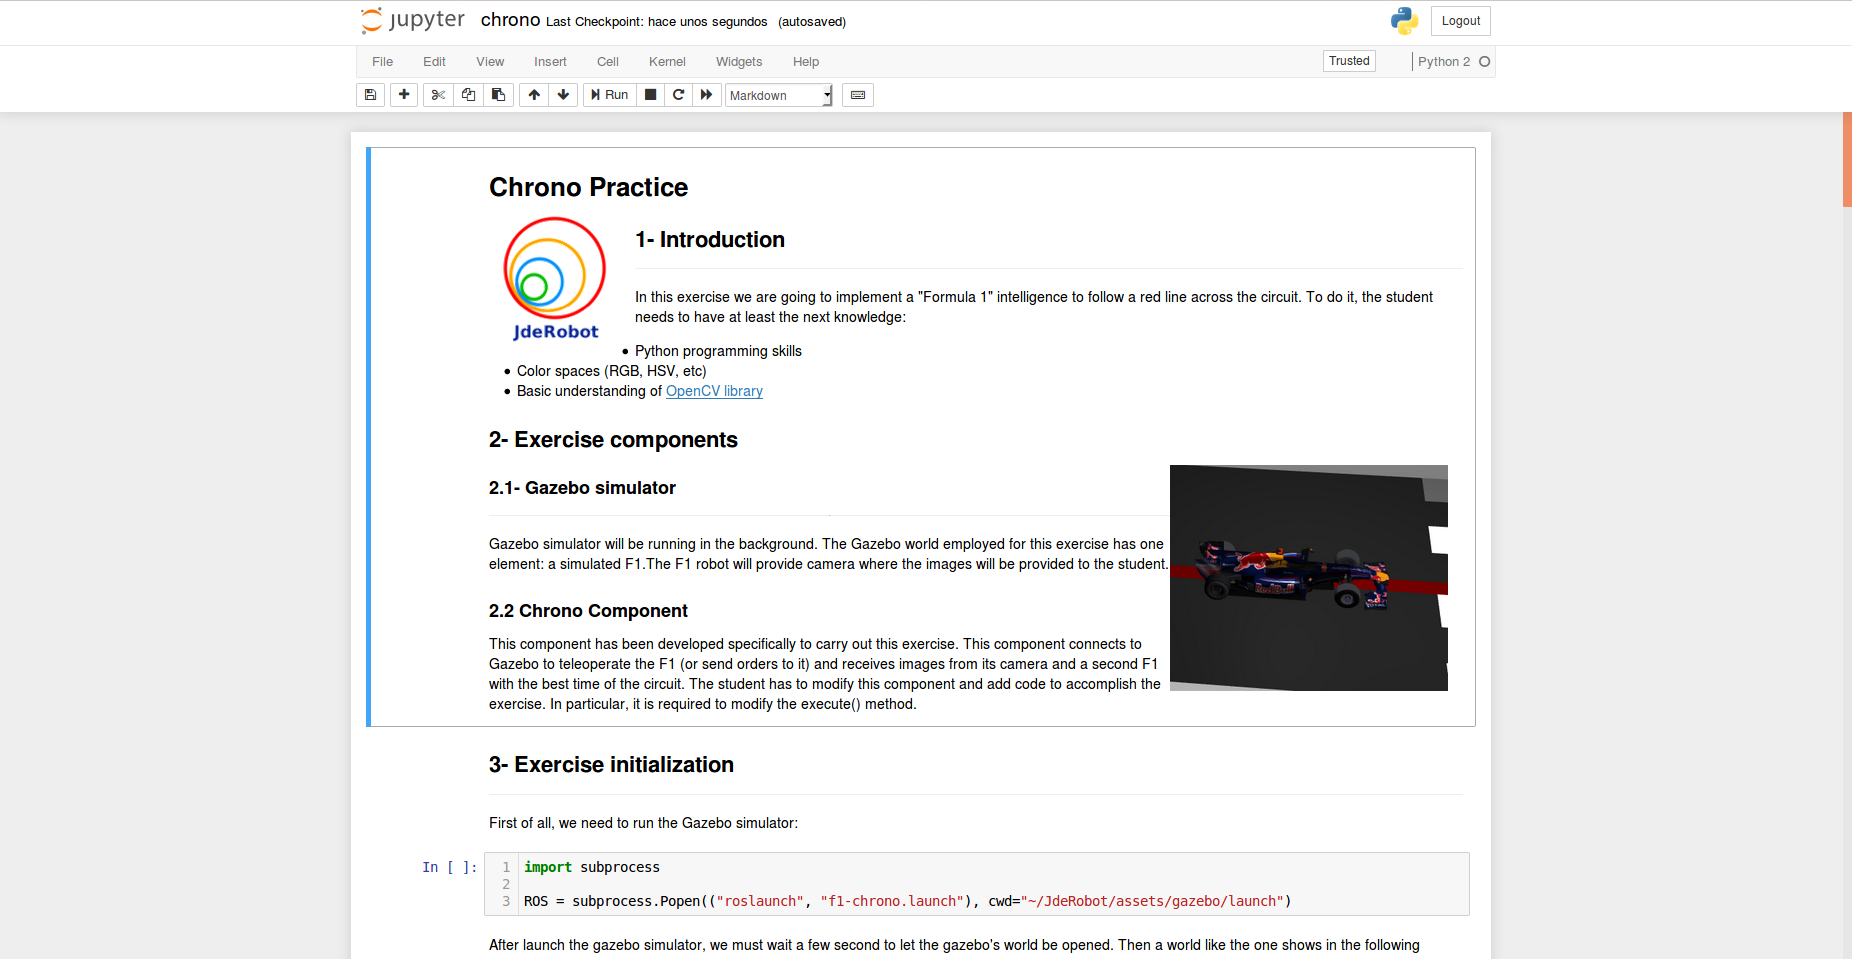
\includegraphics[width=0.98\textwidth]{figures/ipynb_chrono.png}
		\caption{Fichero Chrono.ipynb}
		\label{fig.fcipynb}
		\end{center}
\end{figure}

El alumno deberá ejecutar las celdas con código y seguir el guión mostrado. En primer lugar deberá ejecutar el fichero de configuración del mundo que abrirá el escenario en Gazebo (Figura \ref{fig.cmdc}).

\begin{figure}[H]
  \begin{center}
    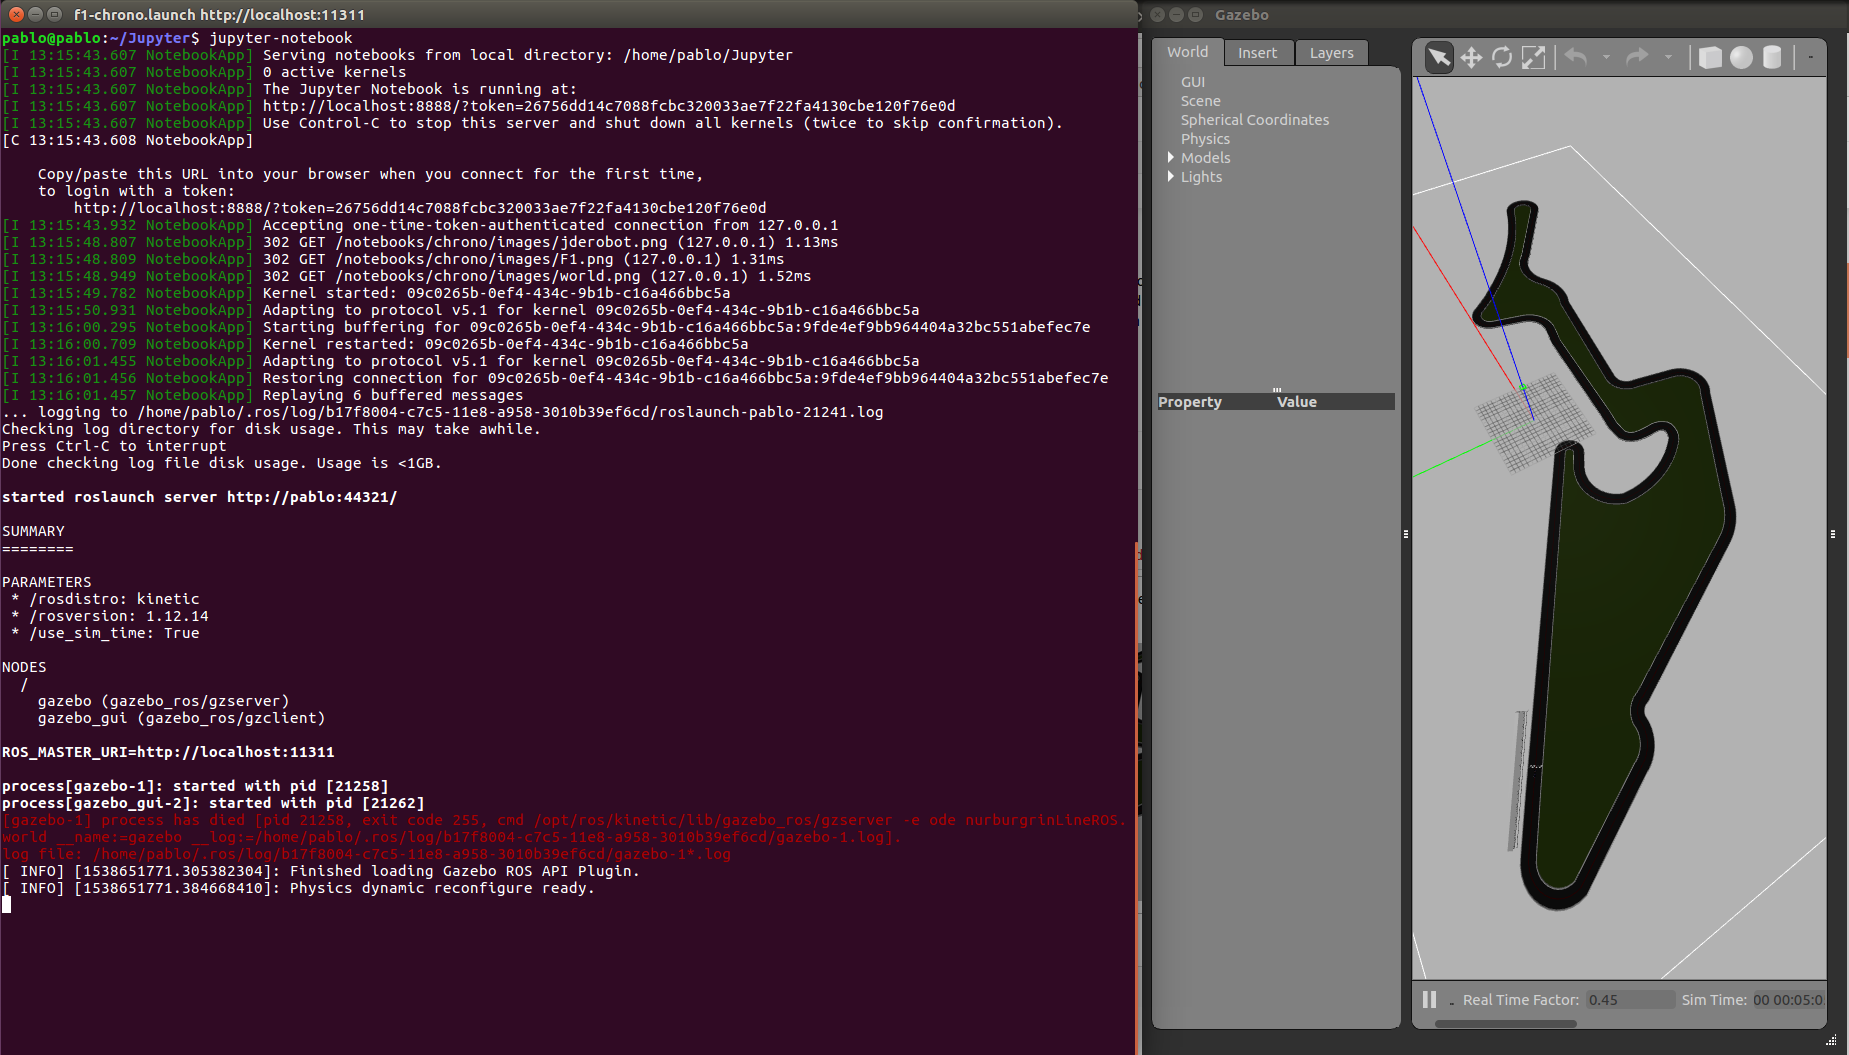
\includegraphics[width=0.98\textwidth]{figures/celda_mundo_chrono.png}
		\caption{Visualización del mundo}
		\label{fig.cmdc}
		\end{center}
\end{figure}

Cuando se haya abierto el simulador es necesario importar el módulo del paquete ``MyAlgorithm.py'' y ``chrono.py'' para tener la funcionalidad provista en el nodo ROS. Para ello, se ejecutará la celda correspondiente con las clases ``MyAlgorithm'' y ``Chrono''. Estas clases son código transparente para el estudiante que, una vez ejecutadas, se ocultarán. Una vez importadas, aparece un mensaje de confirmación (Figura \ref{fig.cmdc}).

\begin{figure}[H]
  \begin{center}
    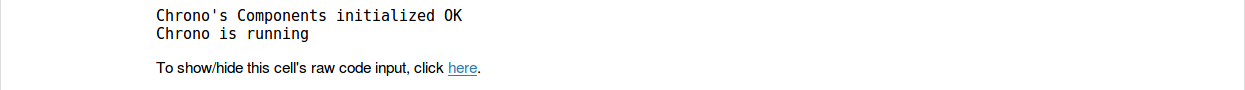
\includegraphics[width=1.5\textwidth]{figures/imp_Ma_CH.png}
		\caption{Importación de las clases ``MyAlgorithm'' y ``Chrono''}
		\label{fig.cmdc}
		\end{center}
\end{figure}


Cuando la ejecución imprima el mensaje ``OK'', el alumno puede comenzar a programar su código en la celda especificada para ello.

\begin{figure}[H]
  \begin{center}
    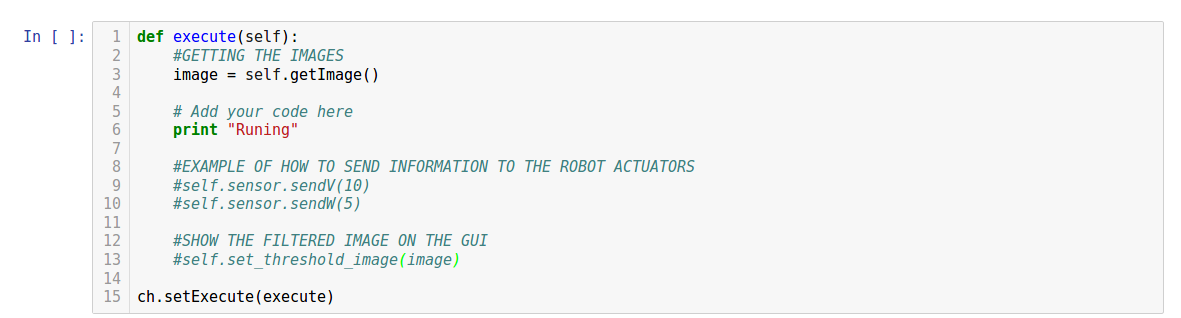
\includegraphics[width=.7\textwidth]{figures/celda_solucion_chrono.png}
		\caption{Celda con el algoritmo del alumno}
		\label{fig.ccach}
		\end{center}
\end{figure}

Para comprobar el código desarrollado, basta con ejecutar la celda donde ha programado el algoritmo. Si quiere parar la ejecución, es suficiente con pulsar el botón con el icono de ``Stop'' del cuadernillo. En este instante, Gazebo sigue recibiendo órdenes de mantener el robot estático. En ese instante, el alumno podrá modificar su código y volver a ejecutar la celda con el código modificado. Estos cambios se verán reflejados en Gazebo en el momento.

\begin{figure}[H]
	\begin{center}
    \centering
    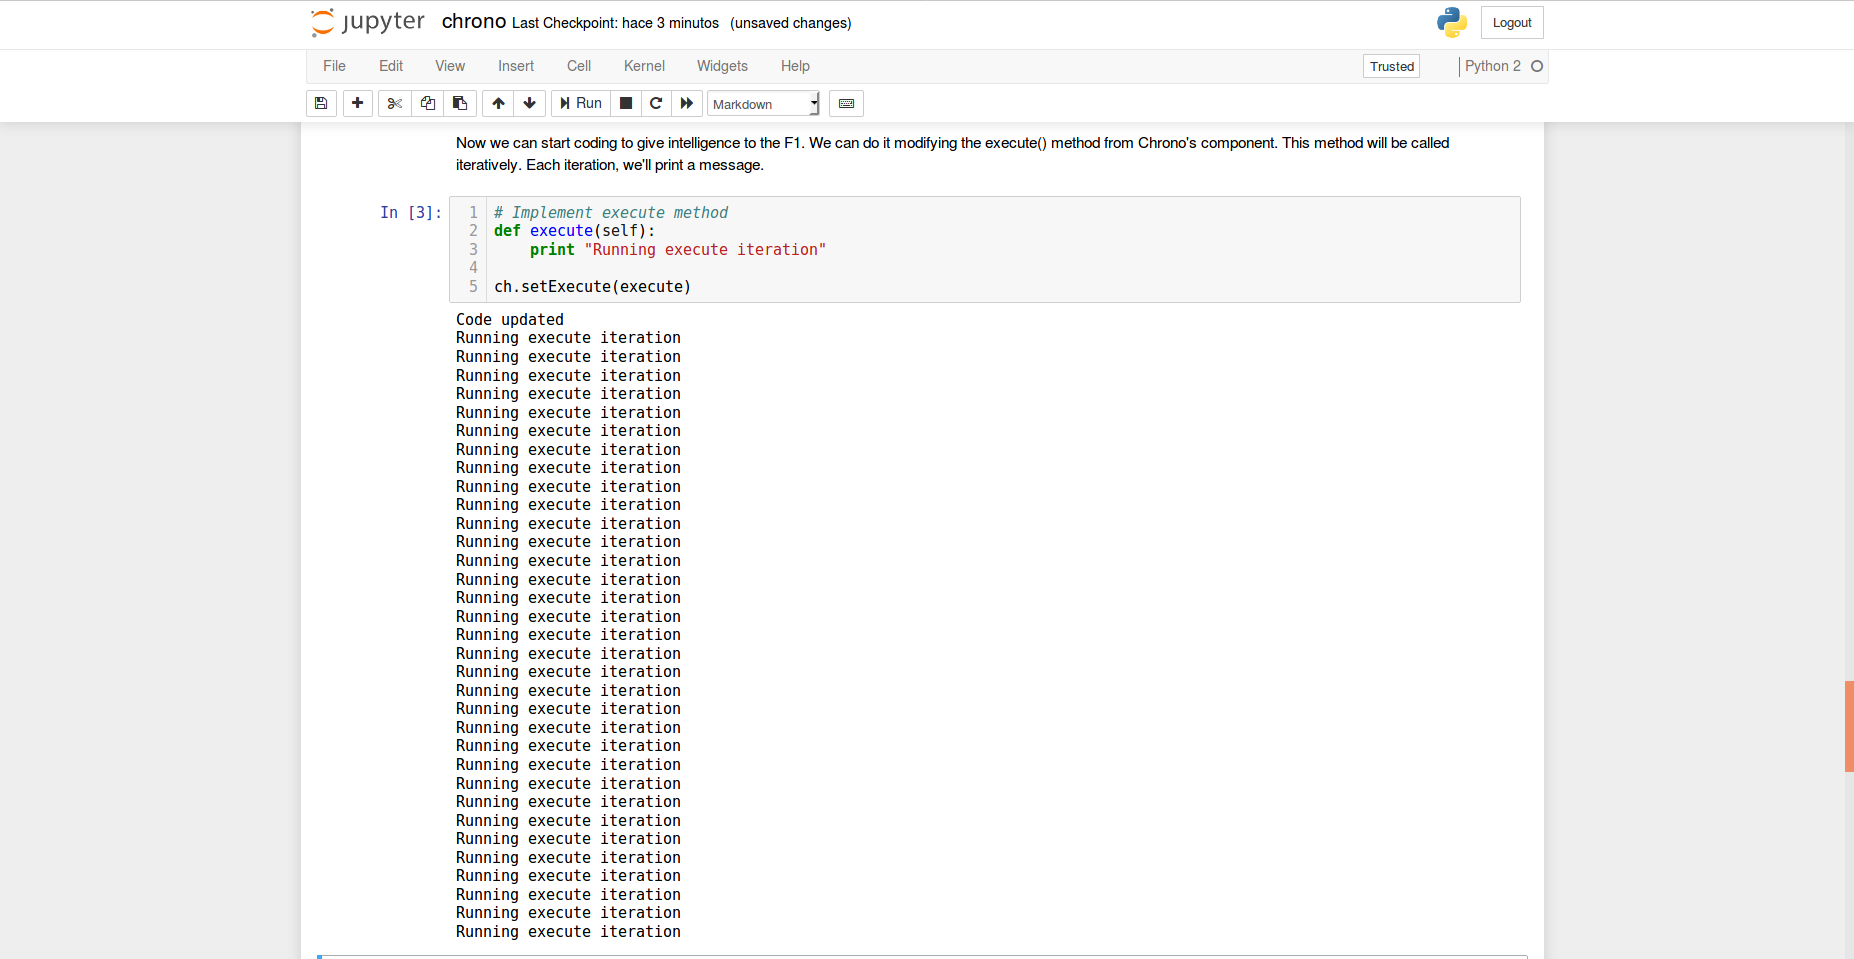
\includegraphics[width=.7\textwidth]{figures/ejecucion_chrono_jupyter.png}
		\caption{Ejecución de la celda del algoritmo}
		\label{fig.ecj}
	\end{center}
\end{figure}

A continuación, se muestran algunas fotos de la ejecución:

\begin{figure}[H]
  \begin{center}
    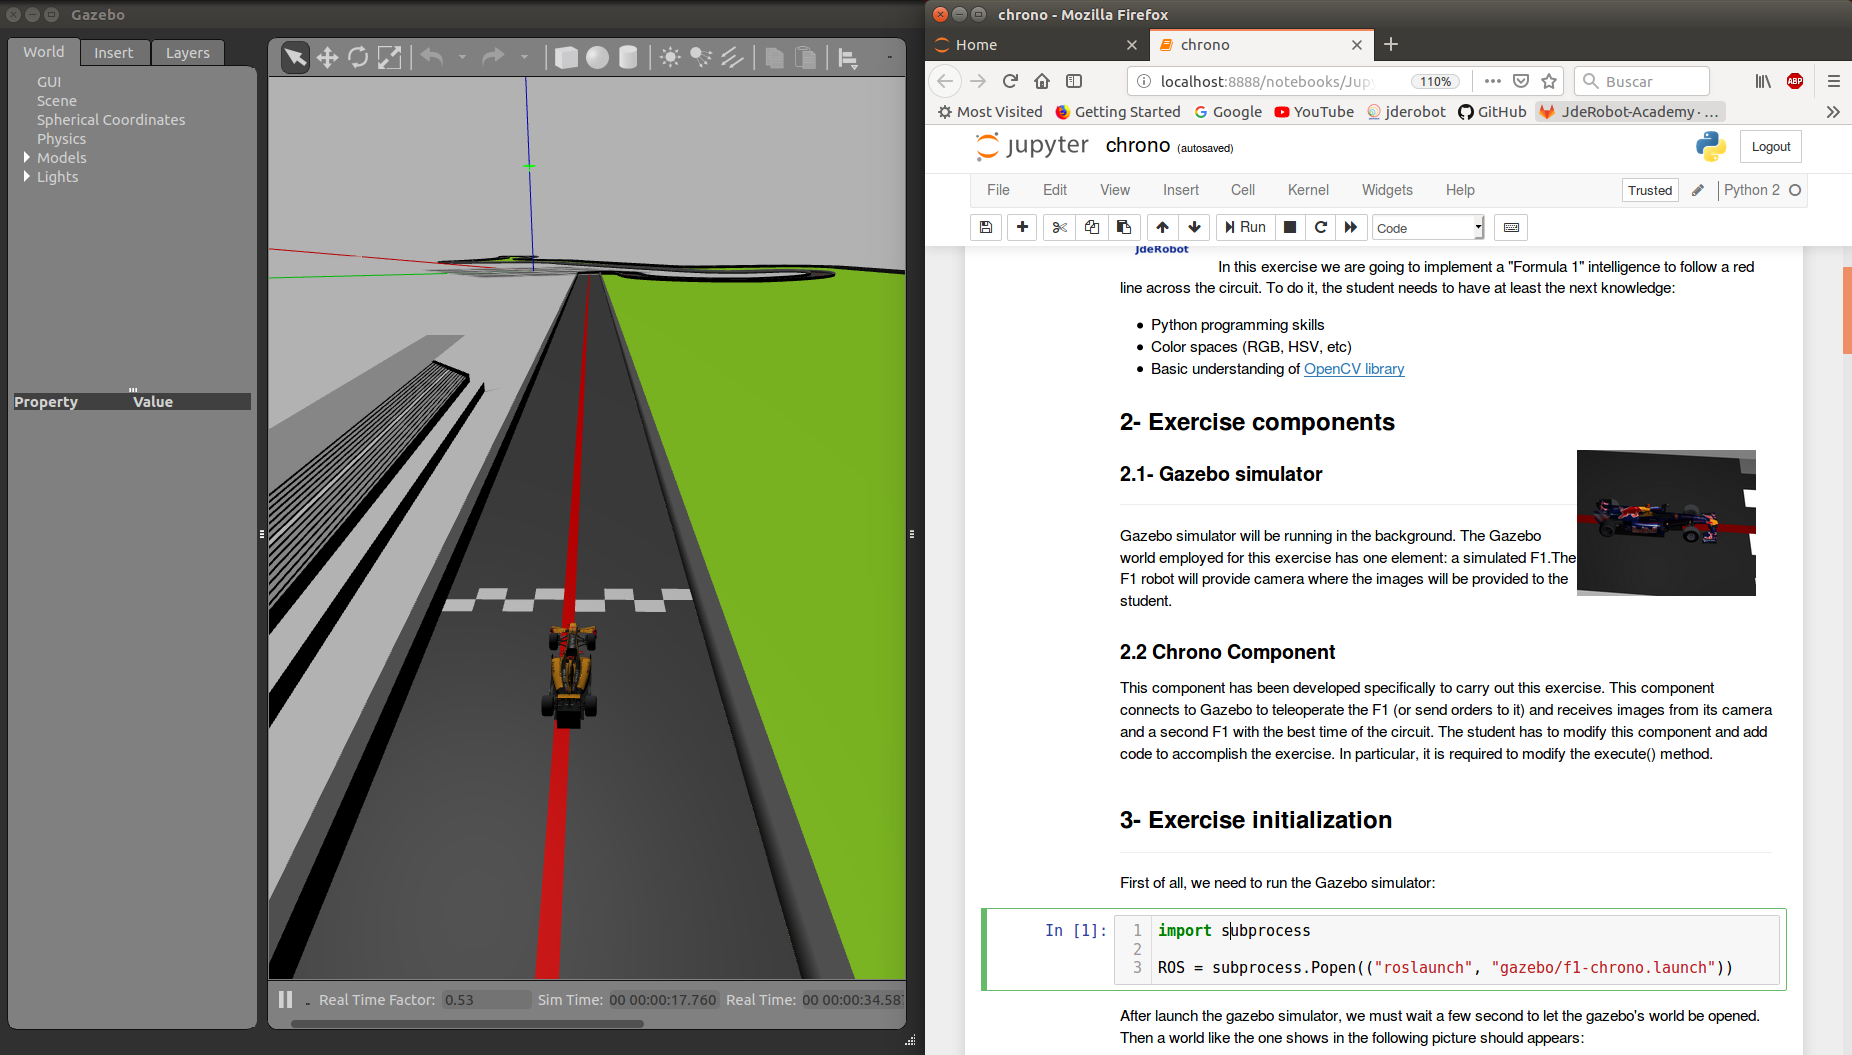
\includegraphics[width=0.9\textwidth]{figures/ejec_1_jup_ch.png}
		\caption{Ejecución del código del ejercicio de Chrono desde un navegador web (a)}
		\label{fig.ecjfr1}
		\end{center}
\end{figure}

\begin{figure}[H]
  \begin{center}
    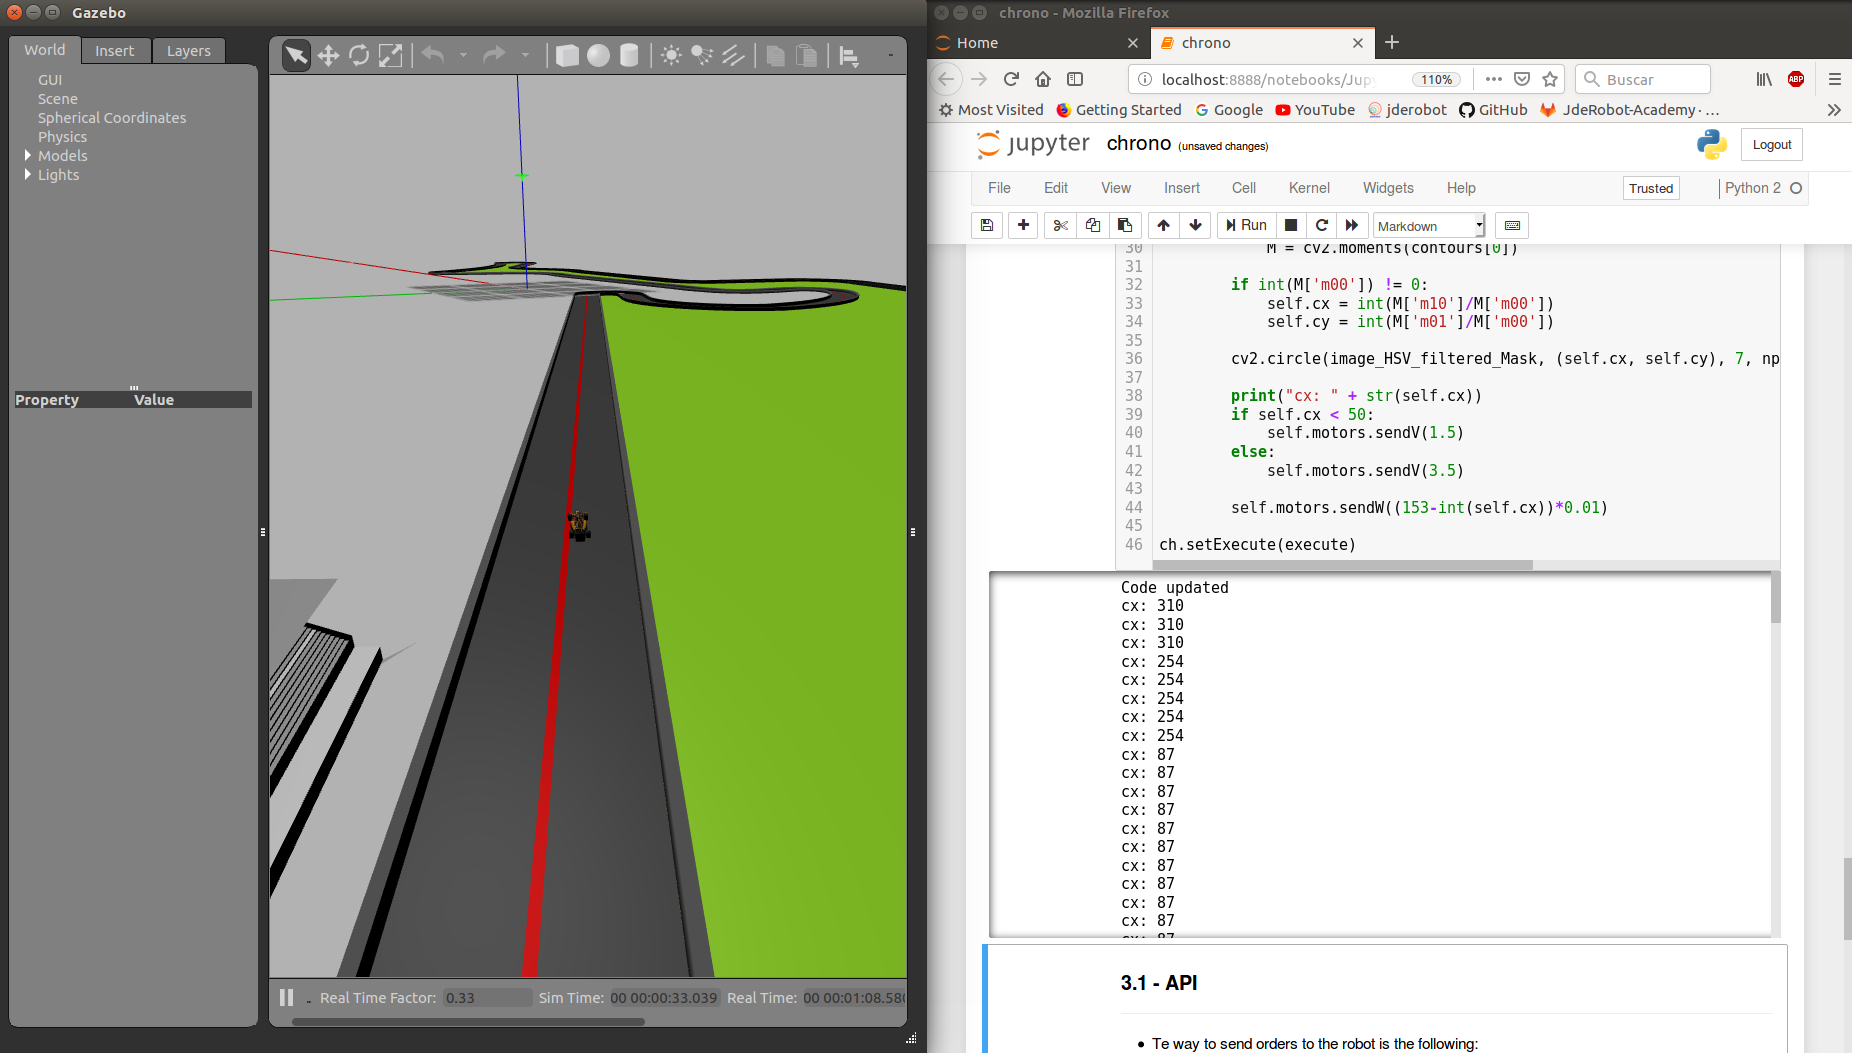
\includegraphics[width=0.9\textwidth]{figures/ejec_2_jup_ch.png}
		\caption{Ejecución del código del ejercicio de Chrono desde un navegador web (b)}
		\label{fig.ecjfr2}
		\end{center}
\end{figure}

\begin{figure}[H]
  \begin{center}
    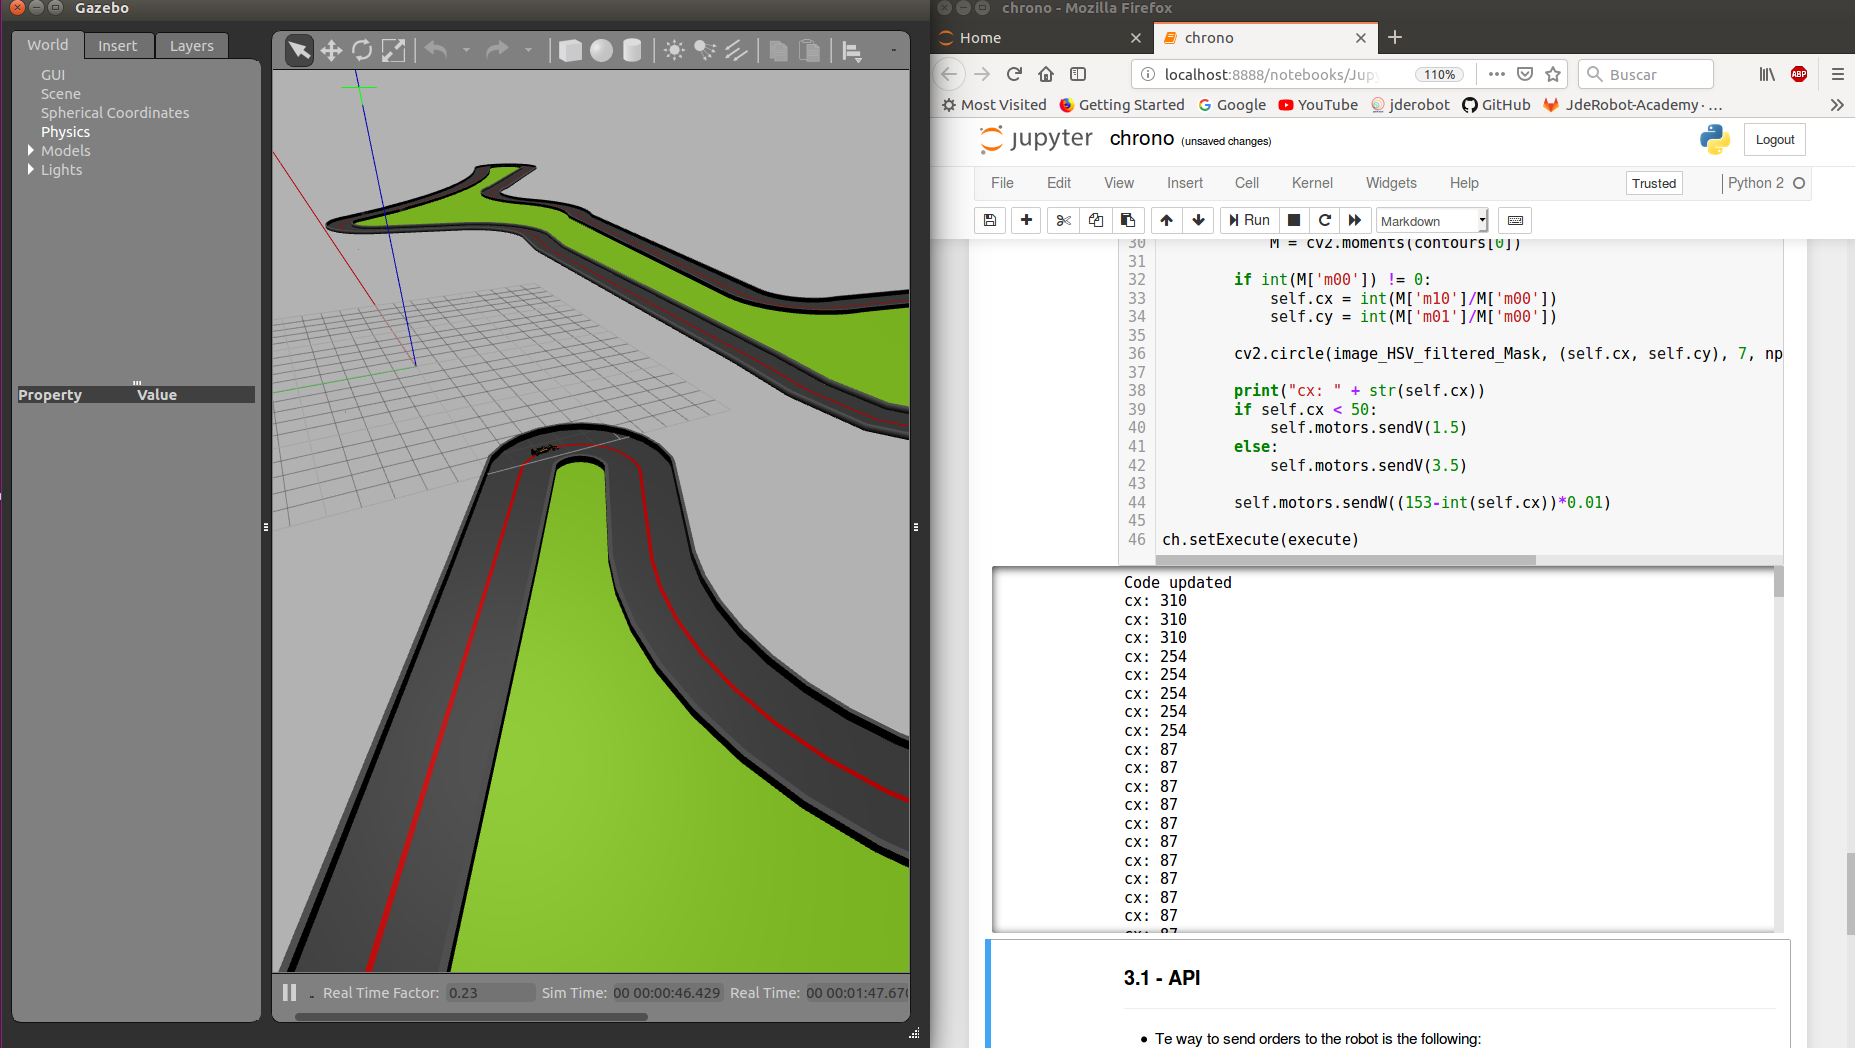
\includegraphics[width=0.9\textwidth]{figures/ejec_3_jup_ch.png}
		\caption{Ejecución del código del ejercicio de Chrono desde un navegador web (c)}
		\label{fig.ecjfr3}
		\end{center}
\end{figure}
